\documentclass{article}

\usepackage{tikz}
\usepackage{minted}
\usepackage{ifthen}
\usepackage{caption}
\usepackage{subfig}
\usepackage{listings}
\usepackage{geometry}
 \geometry{
	 a4paper,
	 left=25mm,
	 right=20mm,
	 top=20mm,
	 bottom=20mm,
 }

\usetikzlibrary{calc,positioning,shadows.blur,decorations.pathreplacing,decorations.pathmorphing}
\usepackage{etoolbox}


\definecolor{r0d}{RGB}{255,214,226}
\definecolor{r1d}{RGB}{165,201,239}
\definecolor{r2d}{RGB}{196,228,239}

\tikzset{%
	snake it/.style = {decorate, decoration=snake},
  brace/.style = { decorate, decoration={brace, amplitude=5pt} },
  mbrace/.style = { decorate, decoration={brace, amplitude=5pt, mirror} },
  label/.style = { black, midway, scale=0.8, align=center },
  toplabel/.style = { label, above=.5em, anchor=south },
  leftlabel/.style = { label,rotate=90,left=1.9em,anchor=north },   
  rightlabel/.style = { label,rotate=-90,right=1.5em,anchor=north },   
  bottomlabel/.style = { label, below=.5em, anchor=north },
  force/.style = { rotate=-90,scale=0.4 },
  round/.style = { rounded corners=2mm },
  legend/.style = { right,scale=0.4 },
  nosep/.style = { inner sep=0pt },
  generation/.style = { anchor=base }
}


\begin{document}

\title{Sparse Matrix-Vector Multiplication with CUDA}
\author{Georgii Evtushenko}

\maketitle

\section{Introduction}

Standard methods of differential equations discretization usually lead to systems of linear equations. 
A general feature of produced systems is that the number of entries in each equation depends on local topological features of the discretization.
Thus, the matrices generated by these systems contain a lot of zeroes (fig. \ref{fem_to_sparse_matrix}). It's possible to take advantage of knowledge about zeroes' position by 
storing matrices in special data structures. The abstract data type for these structures is called the sparse matrix. While I was reading about yet another matrix format,
I decided to actualize the performance comparison of different matrix formats. This post provides an efficiency review for basic sparse matrix data structures in the context 
of sparse matrix-vector multiplication (SpMV) on GPU.

\begin{figure}[H]
  \centering
  \subfloat[Mesh]
  {
    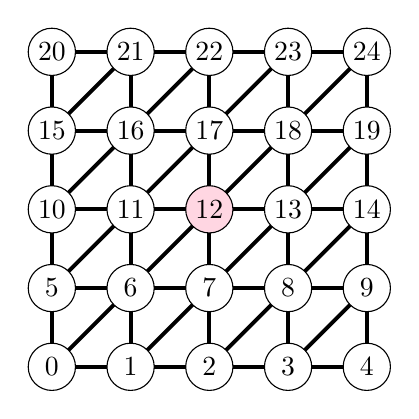
\begin{tikzpicture}[circ/.style = {circle, draw, inner sep=0pt, minimum size=3pt, outer sep=0pt, minimum size=6mm}]
      \pgfmathsetmacro{\lastelementsinrow}{4}
      \foreach \x in {0,...,\lastelementsinrow}
      {
        \foreach \y in {0,...,\lastelementsinrow}
        {
          \pgfmathtruncatemacro{\label}{\y * \lastelementsinrow + \y + \x}
          \ifthenelse{\x=2 \AND \y=2}{\node (\x\y) [circ,fill=r0d] at (\x, \y) {\label}}{\node (\x\y) [circ] at (\x, \y) {\label}};
        }
      }

      \foreach \x in {1,...,\lastelementsinrow}
      {
        \foreach \y in {0,...,\lastelementsinrow}
        {
          \pgfmathtruncatemacro{\px}{\x - 1}
          \draw [line width=0.5mm] (\x\y) -- (\px\y);
        }
      }

      \foreach \x in {0,...,\lastelementsinrow}
      {
        \foreach \y in {1,...,\lastelementsinrow}
        {
          \pgfmathtruncatemacro{\py}{\y - 1}
          \draw [line width=0.5mm] (\x\y) -- (\x\py);
        }
      }

      \foreach \x in {1,...,\lastelementsinrow}
      {
        \foreach \y in {1,...,\lastelementsinrow}
        {
          \pgfmathtruncatemacro{\py}{\y - 1}
          \pgfmathtruncatemacro{\px}{\x - 1}
          \draw [line width=0.5mm] (\x\y) -- (\px\py);
        }
      }
    \end{tikzpicture}
  }
  \qquad
  \subfloat[Matrix]
  {
    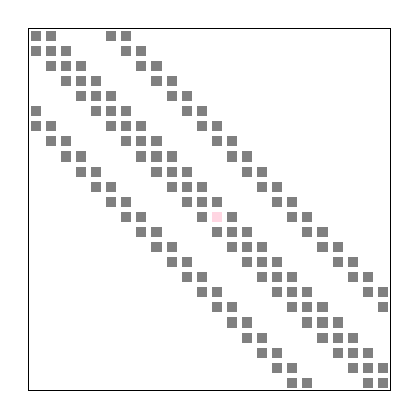
\begin{tikzpicture}
      \pgfmathsetmacro{\size}{4.6}
      \pgfmathsetmacro{\es}{\size/24}
      \pgfmathsetmacro{\pd}{\es/6}
      \pgfmathsetmacro{\ebs}{\es - 2 * \pd}
      \draw (0,0) rectangle ++(\size,\size);

      % Diagonal part
      \foreach \x in {0,...,23}
        \foreach \y in {0,...,23}
         \ifthenelse{\x=\y}
         {
           \ifthenelse{\y=12}
           {
             \fill [r0d] (\es * \x + \pd, \size - \es * \y - \es + \pd) rectangle ++(\ebs, \ebs)
           }
           {
             \fill [gray] (\es * \x + \pd, \size - \es * \y - \es + \pd) rectangle ++(\ebs, \ebs)
           }
         }{};

      % Left part
      \foreach \y in {1,...,23}
       \fill [gray] (\es * \y - \es + \pd, \size - \es * \y - \es + \pd) rectangle ++(\ebs, \ebs);

      % Right part
      \foreach \y in {0,...,22}
       \fill [gray] (\es * \y + \es + \pd, \size - \es * \y - \es + \pd) rectangle ++(\ebs, \ebs);

      % Bottom part
      \foreach \y in {5,...,23}
       \fill [gray] (\es * \y - 5 * \es + \pd, \size - \es * \y - \es + \pd) rectangle ++(\ebs, \ebs);

      % Top part
      \foreach \y in {0,...,18}
       \fill [gray] (\es * \y + 5 * \es + \pd, \size - \es * \y - \es + \pd) rectangle ++(\ebs, \ebs);

      % Diag part
      \foreach \y in {0,...,17}
       \fill [gray] (\es * \y + 6 * \es + \pd, \size - \es * \y - \es + \pd) rectangle ++(\ebs, \ebs);
      \foreach \y in {6,...,23}
       \fill [gray] (\es * \y - 6 * \es + \pd, \size - \es * \y - \es + \pd) rectangle ++(\ebs, \ebs);
    \end{tikzpicture}
  }
  \caption{A simple finite element mesh model}
  \label{fem_to_sparse_matrix}
\end{figure}




\section{Data Structures for Sparse Matrices}
In general, SpMV performance is limited by memory bandwidth. The storage formats used for the sparse matrix define SpMV algorithms. Each of these
algorithms has it's own granularity, which impacts performance. The primary distinction among sparse matrix representations is the 
sparsity pattern, or the structure of the non-zero entries, for which they are best suited. However, I'll start with general sparse matrix formats. 

To access the efficiency of SpMV on different sparse matrix formats, I've collected performance data on general matrices from
Florida Sparse Matrix Collection. All of the experiments are run on a system with NVIDIA RTX 2080 GPU paired with an Intel Core i7-7700k CPU. Each
of the measurements is an average (arithmetic mean) over 30 trials. Before measuring performance, both CPU and GPU frequency were fixed. The speedup is computed
by dividing single thread CSR SpMV execution time by GPU one.




\subsection{CSR}
The \textit{Compressed Sparse Row} (CSR) format is a general sparse matrix format. CSR format consists of three arrays: \textit{row\_ptr},
non-zeroes' \textit{columns}, and matrix \textit{values} (fig. \ref{csr_format}). The row's non-zero values are stored consequentially in an one-dimensional \textit{values} array. The \textit{row\_ptr} array
is used to divide \textit{values} array into separate rows. Its size is equal to $n\_rows + 1$. The last entry in \textit{row\_ptr} stores number of non-zeroes (NNZ) in the
matrix. That allows fast querying of non-zeroes number in a particular row ($row\_ptr[row+1] - row\_ptr[row]$).
For each non-zero value column index is stored in \textit{columns} array.

\begin{figure}[H]
  \centering
  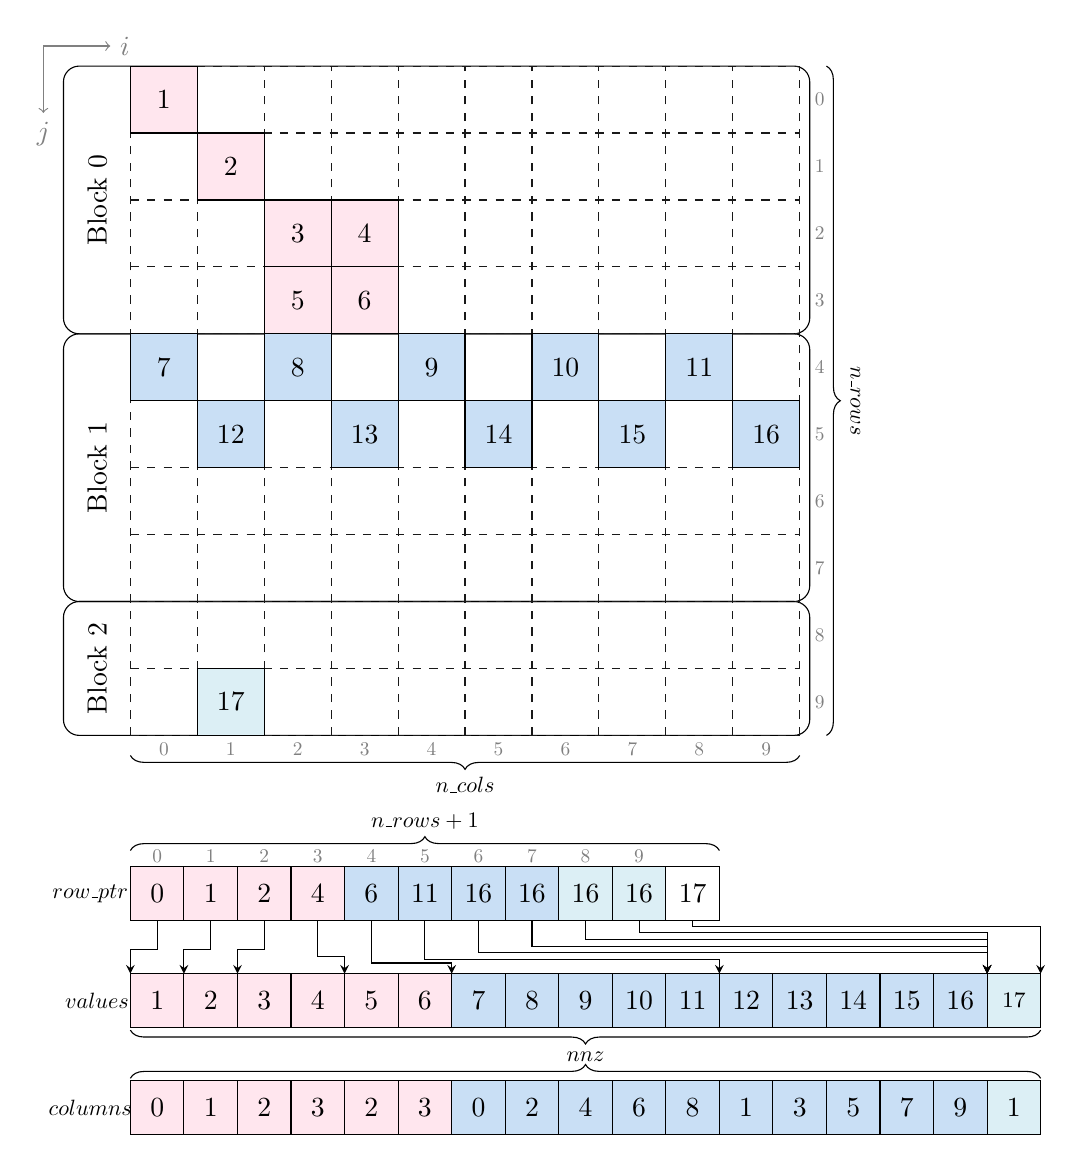
\begin{tikzpicture}[circ/.style = {circle, draw, inner sep=0pt, minimum size=3pt, outer sep=0pt, minimum size=6mm}, scale=0.85]

	\draw[round] (-1.0,0) rectangle (10.15,2.0);
  \draw[round] (-1.0,2.0) rectangle (10.15,6.0);
  \draw[round] (-1.0,6.0) rectangle (10.15,10);

	
  \node[rotate=90] at (-0.5,8)   {Block 0};
  \node[rotate=90] at (-0.5,4.0) {Block 1};
  \node[rotate=90] at (-0.5,1.)  {Block 2};

  \foreach \y in {0,...,9} {
    \node[scale=0.7,text=gray] at (10.3,10.0 - 1.0*\y - 0.5) {\y};
  }

  \foreach \x in {0,...,9} {
    \node[scale=0.7,text=gray] at (1.0*\x + 0.5,-0.2) {\x};
  }

  \draw[->,gray] (-1.3,10.3) -- (-0.3,10.3) node[right] {$i$};
  \draw[->,gray] (-1.3,10.3) -- (-1.3,9.3) node[below] {$j$};

  % Elements mesh
  \draw[step=1.0,black!90!white,thin,dashed,line width=0.4] (0.0,0.0) grid (10.0,10.0);

  % \draw[round] (-0.15,0) rectangle (10.15,10);

  % Right braces
  \draw [mbrace] (10.4,0.0)  -- (10.4,10.0) node[rightlabel] {$n\_rows$};

  % Bottom braces
  \draw [mbrace] (0.0,-0.3) -- (10,-0.3) node[bottomlabel] {$n\_cols$};

  \edef\esize{1.0}

  % ROW 0
  \edef\elementnum{1}
  \foreach \col in {0} {
    \draw[fill=r0d!60] (\col*\esize,9.0) rectangle (\col*\esize+\esize,10) node[pos=.5] {\elementnum};
    \pgfmathparse{int(\elementnum+1)}
    \xdef\elementnum{\pgfmathresult}
  }
  \foreach \col in {1} {
    \draw[fill=r0d!60] (\col*\esize,8.0) rectangle (\col*\esize+\esize,9) node[pos=.5] {\elementnum};
    \pgfmathparse{int(\elementnum+1)}
    \xdef\elementnum{\pgfmathresult}
  }
  \foreach \col in {2,3} {
    \draw[fill=r0d!60] (\col*\esize,7.0) rectangle (\col*\esize+\esize,8) node[pos=.5] {\elementnum};
    \pgfmathparse{int(\elementnum+1)}
    \xdef\elementnum{\pgfmathresult}
  }
  \foreach \col in {2,3} {
    \draw[fill=r0d!60] (\col*\esize,6.0) rectangle (\col*\esize+\esize,7) node[pos=.5] {\elementnum};
    \pgfmathparse{int(\elementnum+1)}
    \xdef\elementnum{\pgfmathresult}
  }

  % ROW 4
  \foreach \col in {0,2,4,6,8} {
    \draw[fill=r1d!60] (\col*\esize,5.0) rectangle (\col*\esize+\esize,6) node[pos=.5] {\elementnum};
    \pgfmathparse{int(\elementnum+1)}
    \xdef\elementnum{\pgfmathresult}
  }

  % ROW 5
  \foreach \col in {1,3,5,7,9} {
    \draw[fill=r1d!60] (\col*\esize,4.0) rectangle (\col*\esize+\esize,5) node[pos=.5] {\elementnum};
    \pgfmathparse{int(\elementnum+1)}
    \xdef\elementnum{\pgfmathresult}
  }

  % ROW 9
  \foreach \col in {1} {
    \draw[fill=r2d!60] (\col*\esize,0.0) rectangle (\col*\esize+\esize,1) node[pos=.5] {\elementnum};
    \pgfmathparse{int(\elementnum+1)}
    \xdef\elementnum{\pgfmathresult}
  }

  % RHS
  \edef\lasty{0}
  \edef\ynum{1}

  % =====================================================
  % ================== Data structures ================== 
  % =====================================================

  % RHS OFFSETS
  \edef\ybot{-1.0}
  \edef\esize{0.8}

  \edef\xnum{0}
  \edef\lastblockoffset{0}
  \edef\lastyoffset{\ybot-\esize*0.8}

  % ROWS NON ZEROS
  \pgfmathparse{\ybot-\esize*2.2}
  \xdef\ybot{\pgfmathresult}

  % MATRIX OFFSETS
  \draw [mbrace] (11 *\esize,\ybot+1.3*\esize)  -- (0*\esize,\ybot+1.3*\esize) node[toplabel] {$n\_rows+1$};

  \node[scale=0.8] at (-0.6,\ybot+\esize/2) {$row\_ptr$};

  \foreach \i in {0,...,9} {
    \node[scale=0.7,text=gray] at (\i * \esize + \esize/2,\ybot+\esize*1.2) {\i};
  }

  \edef\xnum{0}
  \edef\lastblockoffset{0}
  \edef\middlepoint{\ybot-\esize*0.8}

  \foreach \offset in {0,1,2,4,6,11,16,16,16,16,17} {
    \pgfmathparse{\esize*\offset}
    \xdef\lastblockoffset{\pgfmathresult}

    \ifthenelse{\xnum<4}
    { \draw[fill=r0d!60] (\xnum*\esize,\ybot) rectangle (\xnum*\esize+\esize,\ybot+\esize) node[pos=.5] {\offset}; }
    {
      \ifthenelse{\xnum<8}
      { \draw[fill=r1d!60] (\xnum*\esize,\ybot) rectangle (\xnum*\esize+\esize,\ybot+\esize) node[pos=.5] {\offset}; }
      {
        \ifthenelse{\xnum<10}
        { \draw[fill=r2d!60] (\xnum*\esize,\ybot) rectangle (\xnum*\esize+\esize,\ybot+\esize) node[pos=.5] {\offset}; }
        {
          \ifthenelse{\xnum<11}
          { \draw[fill=white] (\xnum*\esize,\ybot) rectangle (\xnum*\esize+\esize,\ybot+\esize) node[pos=.5] {\offset}; }
          { 
          }
        }
      }
    }

    \ifthenelse{\xnum<2}
    { \draw[>=stealth,->] (\xnum*\esize+\esize/2,\ybot) |- (\lastblockoffset,\middlepoint+0.2) -| (\lastblockoffset,\ybot-\esize); }
    {
      \ifthenelse{\xnum<5}
      { \draw[>=stealth,->] (\xnum*\esize+\esize/2,\ybot) |- (\lastblockoffset,\middlepoint-0.1*\xnum+0.4) -| (\lastblockoffset,\ybot-\esize); }
      {
        \ifthenelse{\xnum<15}
        { \draw[>=stealth,->] (\xnum*\esize+\esize/2,\ybot) |- (\lastblockoffset,\middlepoint+0.1*\xnum-0.45) -| (\lastblockoffset,\ybot-\esize); }
        { }
      }
    }

    \pgfmathparse{int(\xnum+1)}
    \xdef\xnum{\pgfmathresult}
  }

  % MATRIX DATA
  \pgfmathparse{\ybot-\esize*2}
  \xdef\ybot{\pgfmathresult}

  \node[scale=0.8] at (-0.5,\ybot+\esize/2) {$values$};

  % Row 0
  \edef\elementnum{1}
  \foreach \i in {0,...,5} {
    \draw[fill=r0d!60]  (\i * \esize,\ybot) rectangle (\i * \esize + \esize,\ybot+\esize) node[pos=0.5] {\elementnum};
    \pgfmathparse{int(\elementnum+1)}
    \xdef\elementnum{\pgfmathresult}
  }

  % Row 4
  \foreach \i in {6,...,10} {
    \draw[fill=r1d!60]  (\i * \esize,\ybot) rectangle (\i * \esize + \esize,\ybot+\esize) node[pos=0.5] {\elementnum};
    \pgfmathparse{int(\elementnum+1)}
    \xdef\elementnum{\pgfmathresult}
  }

  % Row 5
  \foreach \i in {11,...,15} {
    \draw[fill=r1d!60]  (\i * \esize,\ybot) rectangle (\i * \esize + \esize,\ybot+\esize) node[pos=0.5] {\elementnum};
    \pgfmathparse{int(\elementnum+1)}
    \xdef\elementnum{\pgfmathresult}
  }

  % Row 6
  \foreach \i in {16,...,16} {
    \draw[fill=r2d!60]  (\i * \esize,\ybot) rectangle (\i * \esize + \esize,\ybot+\esize) node[pos=0.5] {\footnotesize \elementnum};
    \pgfmathparse{int(\elementnum+1)}
    \xdef\elementnum{\pgfmathresult}
  }

  \draw [mbrace] (0 *\esize,1.01*\ybot)  -- (17*\esize,1.01*\ybot) node[bottomlabel] {$nnz$};
  \draw [mbrace] (17 *\esize,1.01*\ybot-0.9*\esize) -- (0* \esize,1.01*\ybot-0.9*\esize) node[bottomlabel] {};

  \pgfmathparse{\ybot-\esize*2}
  \xdef\ybot{\pgfmathresult}
  \node[scale=0.8] at (-0.6,\ybot+\esize/2) {$columns$};

  \edef\elementnum{0}
  \foreach \i in {0,1,2,3,2,3} {
    \draw[fill=r0d!60] (\elementnum * \esize,\ybot) rectangle (\elementnum * \esize + \esize,\ybot+\esize) node[pos=0.5] {\i};
    \pgfmathparse{int(\elementnum+1)}
    \xdef\elementnum{\pgfmathresult}
  }
  \foreach \i in {0,2,4,6,8,1,3,5,7,9} {
    \draw[fill=r1d!60] (\elementnum * \esize,\ybot) rectangle (\elementnum * \esize + \esize,\ybot+\esize) node[pos=0.5] {\i};
    \pgfmathparse{int(\elementnum+1)}
    \xdef\elementnum{\pgfmathresult}
  }
  \foreach \i in {1} {
    \draw[fill=r2d!60] (\elementnum * \esize,\ybot) rectangle (\elementnum * \esize + \esize,\ybot+\esize) node[pos=0.5] {\i};
    \pgfmathparse{int(\elementnum+1)}
    \xdef\elementnum{\pgfmathresult}
  }

  \end{tikzpicture}
  \caption{Example of Compressed Sparse Row (CSR) matrix format}
  \label{csr_format}
\end{figure}

Let's assume for simplicity that there are four threads in each CUDA thread block. General CSR SpMV implementation works at the granularity 
of threads per row (fig. \ref{csr_format_work_distribution}). Hence, the matrix in figure \ref{csr_format} is processed by three thread blocks. 
This implementation is usually referenced as CSR-Scalar (list. \ref{csr_scalar}).

\begin{figure}[H]
  \centering
  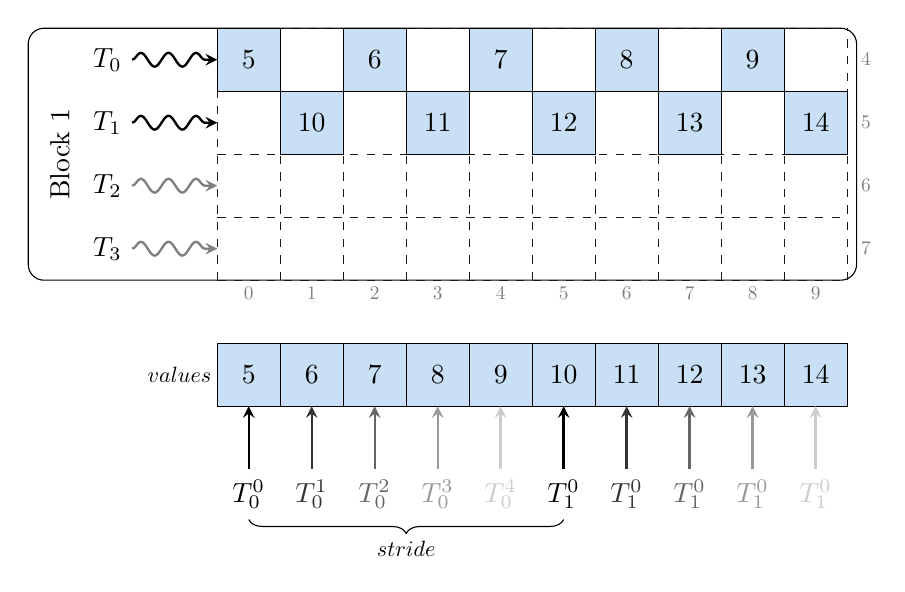
\begin{tikzpicture}[circ/.style = {circle, draw, inner sep=0pt, minimum size=3pt, outer sep=0pt, minimum size=6mm}, scale=0.8]

  \draw[round] (-3.0,2.0) rectangle (10.15,6.0);
  \node[rotate=90] at (-2.5,4.0) {Block 1};

	\draw[draw=black,snake it,line width=0.30mm,>=stealth,->]   (-1.35,5.5) node [anchor=east] {$T_0$} -- (0,5.5);
	\draw[draw=black,snake it,line width=0.30mm,>=stealth,->]   (-1.35,4.5) node [anchor=east] {$T_1$} -- (0,4.5);
	\draw[draw=gray,snake it,line width=0.30mm,>=stealth,->] (-1.35,3.5) node [anchor=east] {$T_2$} -- (0,3.5);
	\draw[draw=gray,snake it,line width=0.30mm,>=stealth,->] (-1.35,2.5) node [anchor=east] {$T_3$} -- (0,2.5);

  \foreach \y in {4,...,7} {
    \node[scale=0.7,text=gray] at (10.3,10.0 - 1.0*\y - 0.5) {\y};
  }

  \foreach \x in {0,...,9} {
    \node[scale=0.7,text=gray] at (1.0*\x + 0.5,1.8) {\x};
  }

  % Elements mesh
  \draw[step=1.0,black!90!white,thin,dashed,line width=0.4] (0.0,2.0) grid (10.0,6.0);

  \edef\esize{1.0}

  % ROW 0
  \edef\elementnum{5}

  % ROW 4
  \foreach \col in {0,2,4,6,8} {
    \draw[fill=r1d!60] (\col*\esize,5.0) rectangle (\col*\esize+\esize,6) node[pos=.5] {\elementnum};
    \pgfmathparse{int(\elementnum+1)}
    \xdef\elementnum{\pgfmathresult}
  }

  % ROW 5
  \foreach \col in {1,3,5,7,9} {
    \draw[fill=r1d!60] (\col*\esize,4.0) rectangle (\col*\esize+\esize,5) node[pos=.5] {\elementnum};
    \pgfmathparse{int(\elementnum+1)}
    \xdef\elementnum{\pgfmathresult}
  }

  % Data access
  \pgfmathparse{2-\esize*2}
  \xdef\ybot{\pgfmathresult}

  \node[scale=0.8] at (-0.6,\ybot+\esize/2) {$values$};

  % Row 0
  \edef\elementnum{5}

  % Row 4
  \foreach \i in {0,...,4} {
    \draw[fill=r1d!60]  (\i * \esize,\ybot) rectangle (\i * \esize + \esize,\ybot+\esize) node[pos=0.5] {\elementnum};
    \pgfmathparse{int(\elementnum+1)}
    \xdef\elementnum{\pgfmathresult}
  }

	\draw[draw=black!100,line width=0.30mm,>=stealth,->] (\esize/2,\ybot-\esize) node [anchor=north] {$T_0^0$} -- (\esize/2,\ybot);
	\draw[draw=black!80,text=black!80,line width=0.30mm,>=stealth,->] (\esize+\esize/2,\ybot-\esize) node [anchor=north] {$T_0^1$} -- (\esize+\esize/2,\ybot);
	\draw[draw=black!60,text=black!60,line width=0.30mm,>=stealth,->] (2*\esize+\esize/2,\ybot-\esize) node [anchor=north] {$T_0^2$} -- (2*\esize+\esize/2,\ybot);
	\draw[draw=black!40,text=black!40,line width=0.30mm,>=stealth,->] (3*\esize+\esize/2,\ybot-\esize) node [anchor=north] {$T_0^3$} -- (3*\esize+\esize/2,\ybot);
	\draw[draw=black!20,text=black!20,line width=0.30mm,>=stealth,->] (4*\esize+\esize/2,\ybot-\esize) node [anchor=north] {$T_0^4$} -- (4*\esize+\esize/2,\ybot);

  % Row 5
  \foreach \i in {5,...,9} {
    \draw[fill=r1d!60]  (\i * \esize,\ybot) rectangle (\i * \esize + \esize,\ybot+\esize) node[pos=0.5] {\elementnum};
    \pgfmathparse{int(\elementnum+1)}
    \xdef\elementnum{\pgfmathresult}
  }

	\draw[draw=black!100,line width=0.30mm,>=stealth,->] (5*\esize+\esize/2,\ybot-\esize) node [anchor=north] {$T_1^0$} -- (5*\esize+\esize/2,\ybot);
	\draw[draw=black!80,text=black!80,line width=0.30mm,>=stealth,->]  (6*\esize+\esize/2,\ybot-\esize) node [anchor=north] {$T_1^0$} -- (6*\esize+\esize/2,\ybot);
	\draw[draw=black!60,text=black!60,line width=0.30mm,>=stealth,->]  (7*\esize+\esize/2,\ybot-\esize) node [anchor=north] {$T_1^0$} -- (7*\esize+\esize/2,\ybot);
	\draw[draw=black!40,text=black!40,line width=0.30mm,>=stealth,->]  (8*\esize+\esize/2,\ybot-\esize) node [anchor=north] {$T_1^0$} -- (8*\esize+\esize/2,\ybot);
	\draw[draw=black!20,text=black!20,line width=0.30mm,>=stealth,->]  (9*\esize+\esize/2,\ybot-\esize) node [anchor=north] {$T_1^0$} -- (9*\esize+\esize/2,\ybot);

  \draw [mbrace] (\esize/2,\ybot-1.8*\esize) -- (5*\esize+\esize/2,\ybot-1.8*\esize) node[bottomlabel] {$stride$};

  \end{tikzpicture}
  \caption{CSR-Scalar block's threads' work distribution}
  \label{csr_format_work_distribution}
\end{figure}

\begin{listing}[H]
\begin{minted}[linenos,tabsize=2]{cuda}
template <typename data_type>
__global__ void csr_spmv_kernel (
		unsigned int n_rows,
		const unsigned int *col_ids,
		const unsigned int *row_ptr,
		const data_type *data,
		const data_type *x,
		data_type *y)
{
	unsigned int row = blockIdx.x * blockDim.x + threadIdx.x;

	if (row < n_rows)
	{
		const int row_start = row_ptr[row];
		const int row_end = row_ptr[row + 1];

		data_type sum = 0;
		for (unsigned int element = row_start; element < row_end; element++)
			sum += data[element] * x[col_ids[element]];
		y[row] = sum;
	}
}
\end{minted}
\caption{Naive SpMV kernel for the CSR-Scalar sparse matrix format}
\label{csr_scalar}
\end{listing}

Presented implementation of CSR SpMV algorithm on GPU is usually considered very inefficient. The reasons for
inefficiency are load balancing, thread divergence, and memory access pattern. As shown in figure \ref{csr_format_work_distribution}, only half
of the block threads have non-zeroes to process. Thus, a single dense row can arbitrarily delay the execution while all
other cores are idle. Moreover, as shown in figure \ref{csr_format_work_distribution}, adjacent threads access matrix values in a strided way. When concurrent threads simultaneously 
access memory addresses that are far apart in physical memory, then there is no chance for the hardware to combine the accesses. Performance
results for naive CSR-Scalar implementation are presented in table \ref{csr_scalar_speedup_table}. 

\begin{table}[H]
	\centering
	\begin{tabular}{ |p{2.6cm}||p{1cm}|p{1cm}|p{1cm}|p{1cm}|  }
	 \hline
		& \multicolumn{2}{|c|}{float} & \multicolumn{2}{|c|}{double}\\
	 \hline
	 NNZ lower limit & avg & max & avg & max  \\
	 \hline
	 10000  & 4.57 & 32.50 & 3.78 & 29.47 \\
	 100000 & 8.90 & 32.50 & 7.24 & 29.47 \\
	 \hline
	\end{tabular}
	\caption{CSR-Scalar speedup}
  \label{csr_scalar_speedup_table}
\end{table}

The speedup distribution is shown in figures \ref{csr_scalar_speedup_float} and \ref{csr_scalar_speedup_double}. To answer the question
how naive described implementation really is I've compared it with the NVIDIA CUDA Sparse Matrix library (cuSPARSE) CSR implementation
(tab. \ref{csr_cusparse_speedup_table}), which has a better average speedup (fig. \ref{csr_cusparse_speedup_float} and \ref{csr_cusparse_speedup_double}). 

\begin{table}[H]
	\centering
	\begin{tabular}{ |p{2.6cm}||p{1cm}|p{1cm}|p{1cm}|p{1cm}|  }
	 \hline
		& \multicolumn{2}{|c|}{float} & \multicolumn{2}{|c|}{double}\\
	 \hline
	 NNZ lower limit & avg & max & avg & max  \\
	 \hline
	 10000  & 5.69  & 31.44 & 4.68 & 25.42 \\
	 100000 & 13.62 & 31.44 & 10.65 & 25.42 \\
	 \hline
	\end{tabular}
	\caption{CSR (cuSPARSE) speedup}
  \label{csr_cusparse_speedup_table}
\end{table}

\begin{figure}[H]
\centering
\subfloat[CSR-Scalar speedup (float) \label{csr_scalar_speedup_float}]  {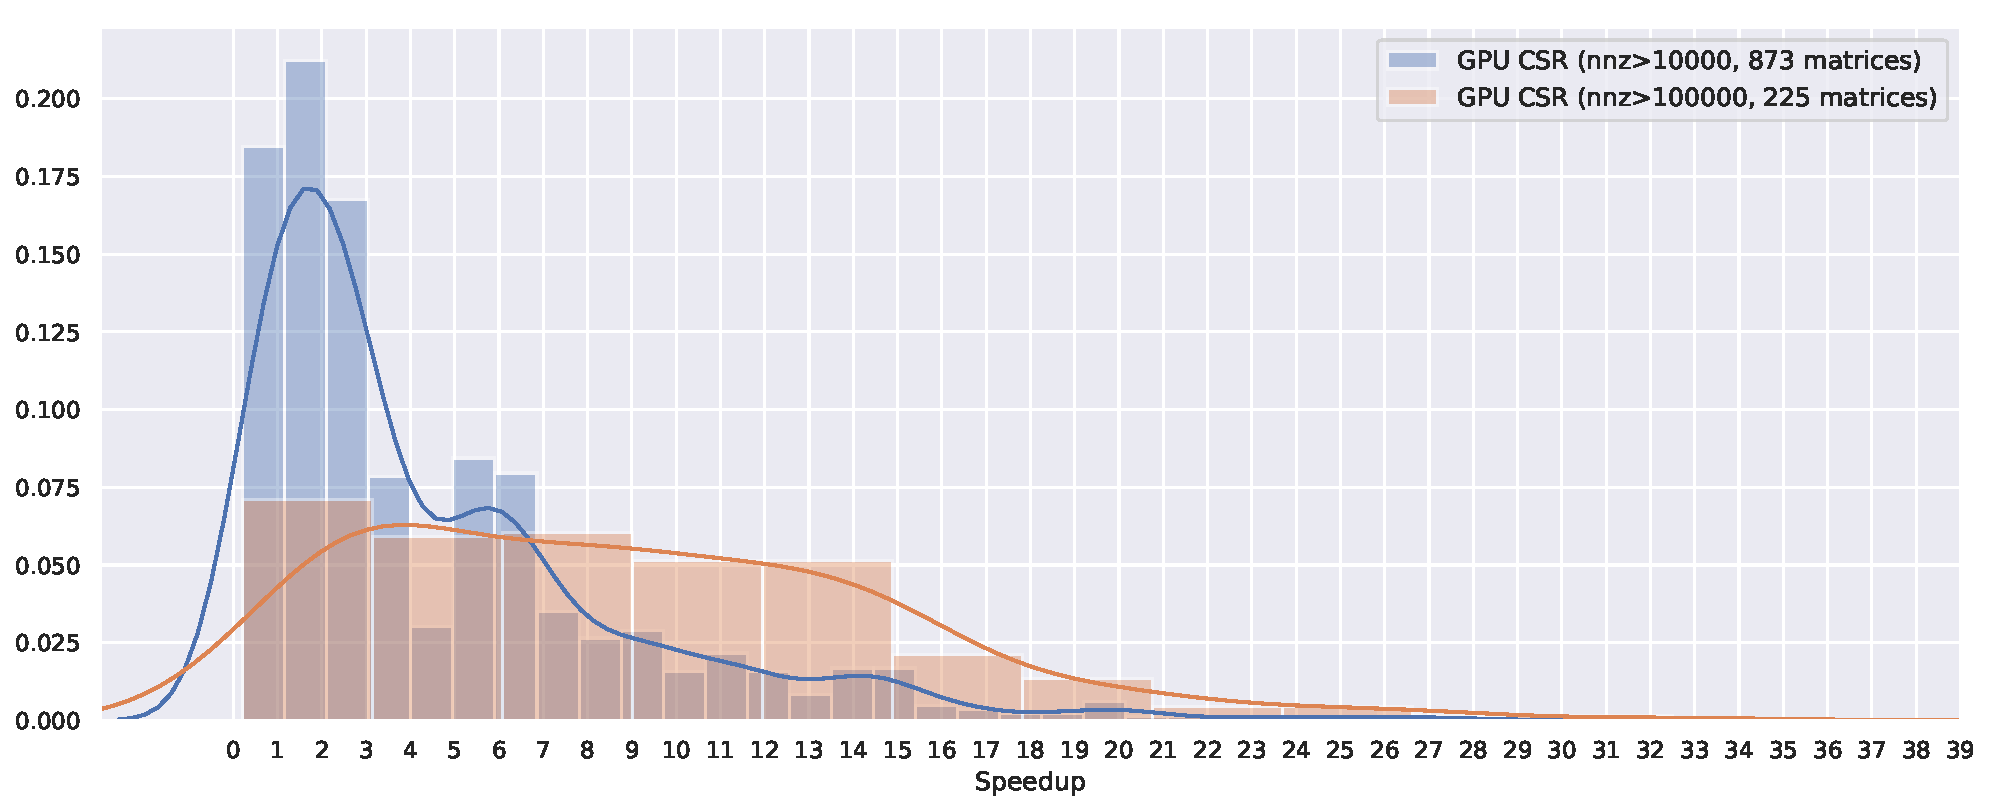
\includegraphics[width=1.0\textwidth]{img/csr_float_dist.pdf}}
\qquad %
\subfloat[CSR-Scalar speedup (double) \label{csr_scalar_speedup_double}] {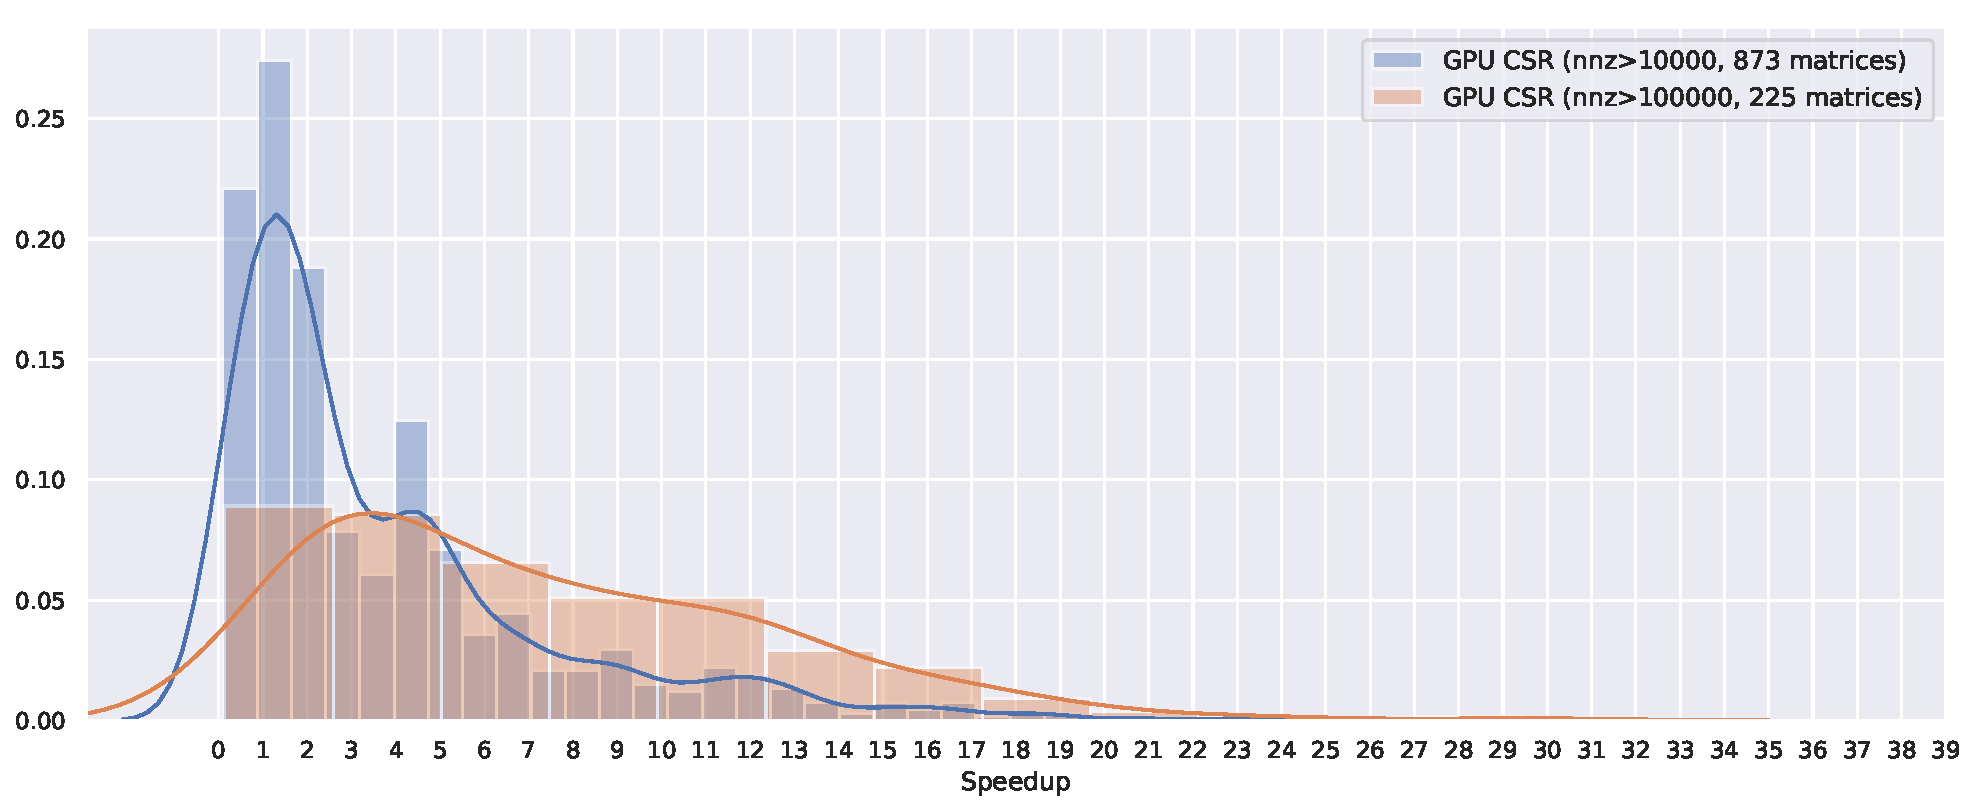
\includegraphics[width=1.0\textwidth]{img/csr_double_dist.pdf}}
\end{figure}

These results show that there is room for optimization of CSR SpMV. The first possible optimization is to assign warp per row instead of thread.
This algorithm (list. \ref{csr_vector}) is called CSR-Vector. The vector kernel accesses indices and data contiguously (fig. \ref{csr_vector_format_mem_access_pattern}), 
and therefore overcomes the principal deficiency of the scalar approach. Unlike the previous CSR implementation, which used one thread per matrix row, this optimization requires
coordination among threads within the same warp. 

\begin{figure}[H]
\centering
\subfloat[CSR cuSPARSE speedup (float) \label{csr_cusparse_speedup_float}]  {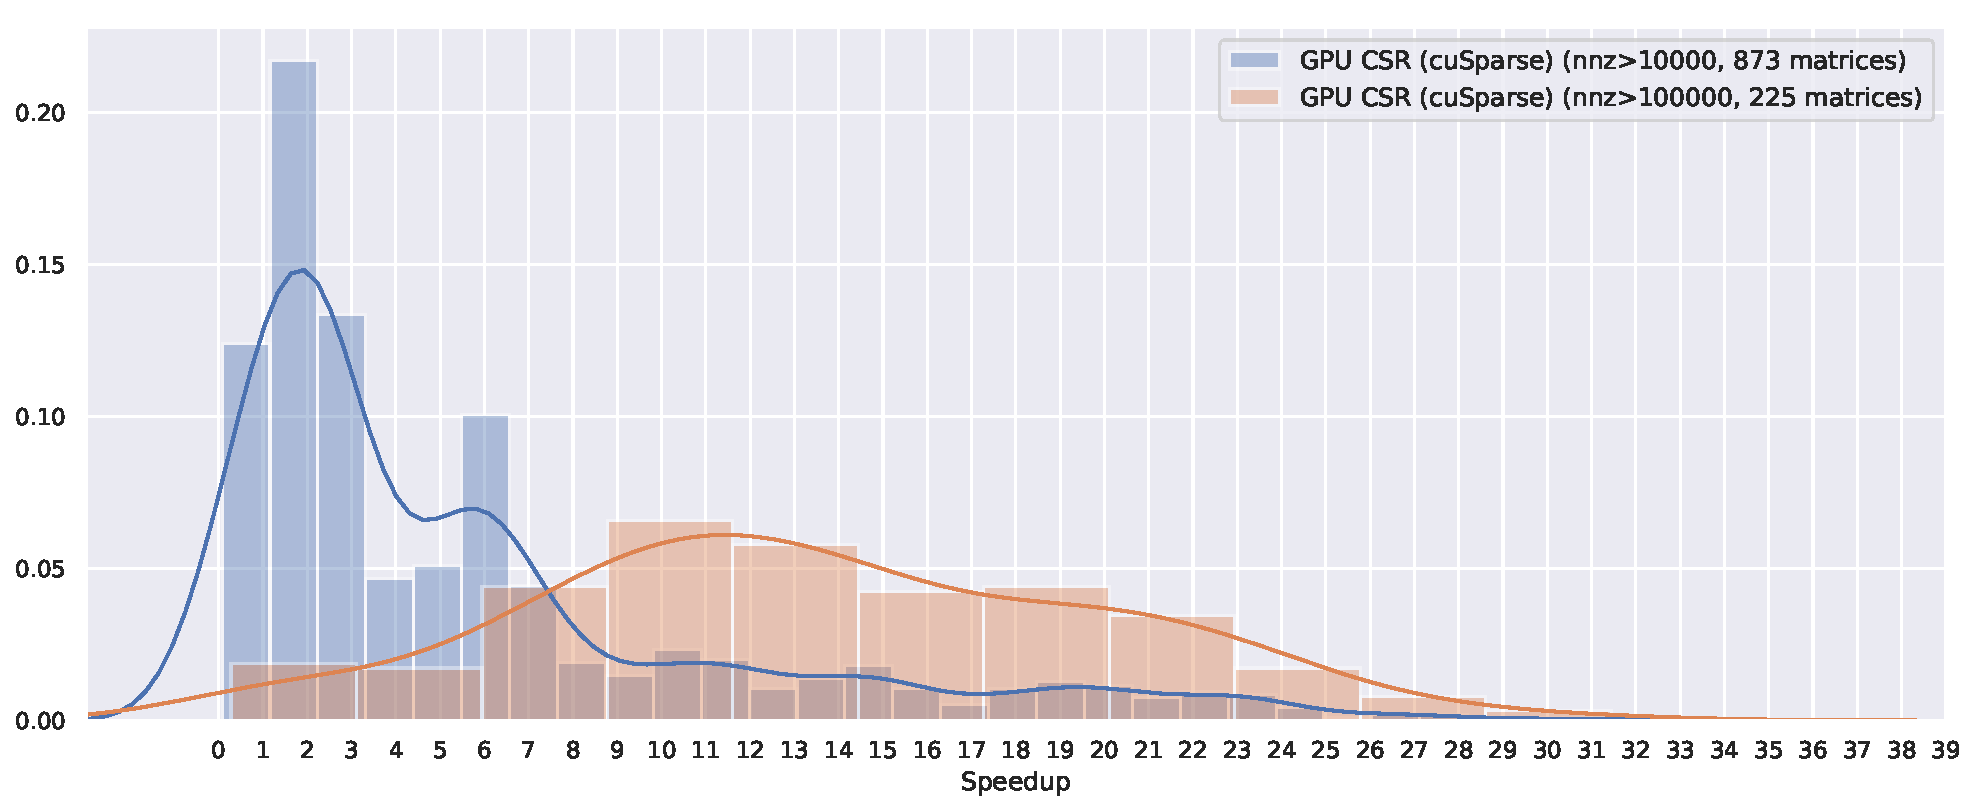
\includegraphics[width=1.0\textwidth]{img/csr_cusparse_float_dist.pdf}}
\qquad %
\subfloat[CSR cuSPARSE speedup (double) \label{csr_cusparse_speedup_double}] {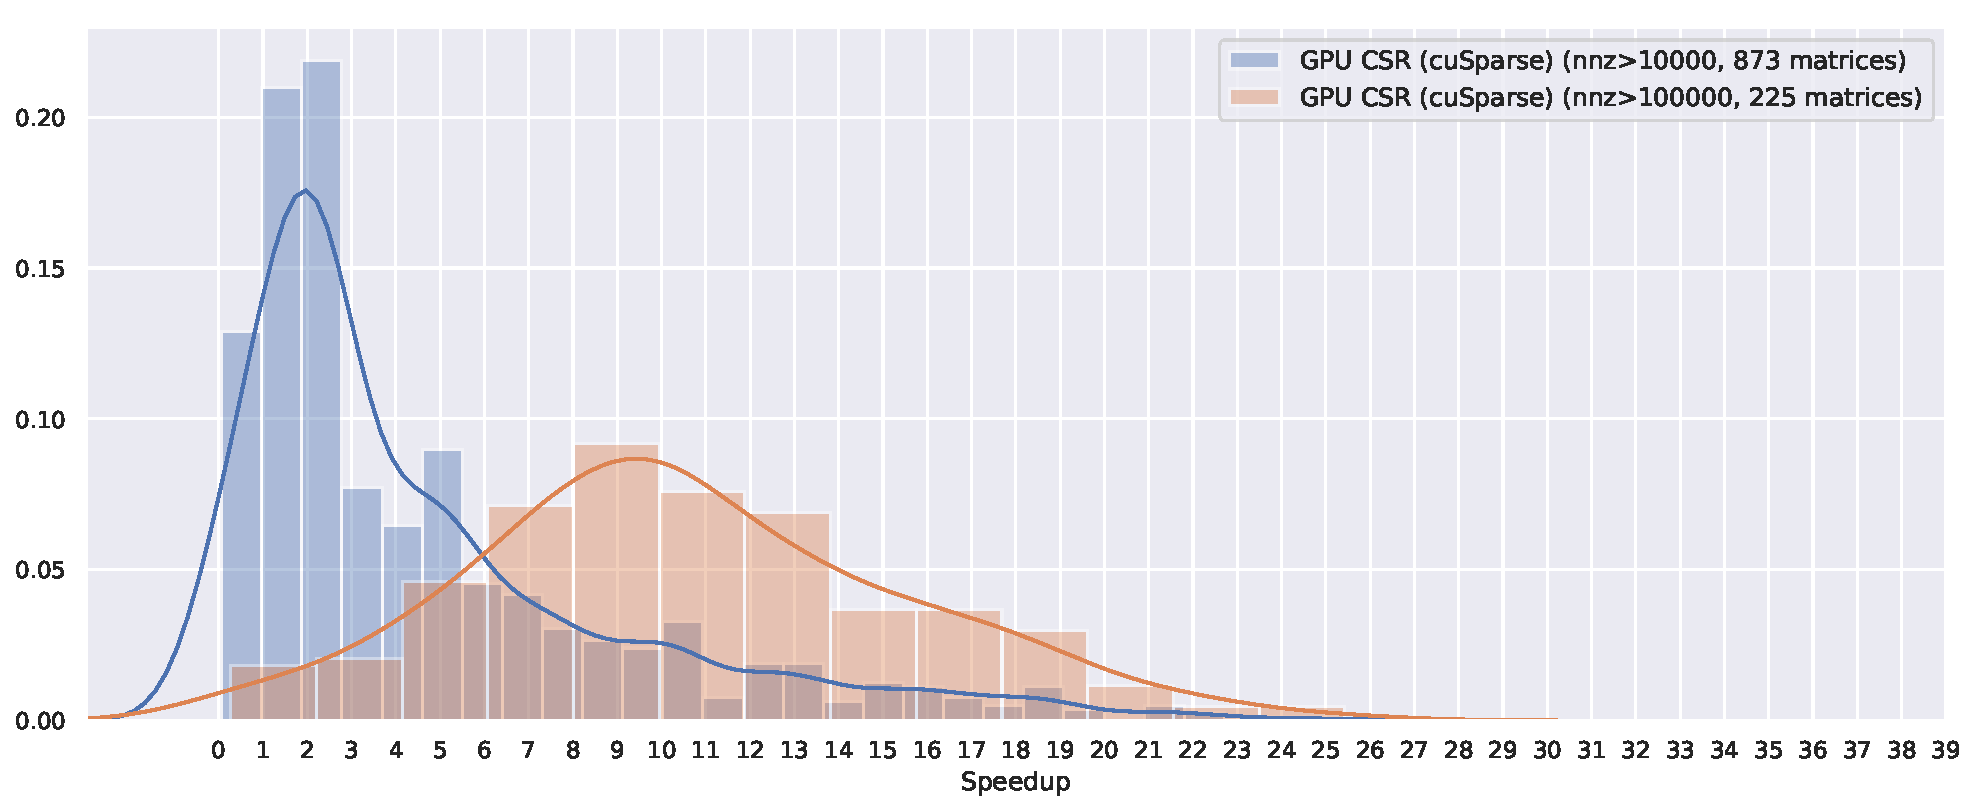
\includegraphics[width=1.0\textwidth]{img/csr_cusparse_double_dist.pdf}}
\end{figure}

\begin{figure}[H]
  \centering
  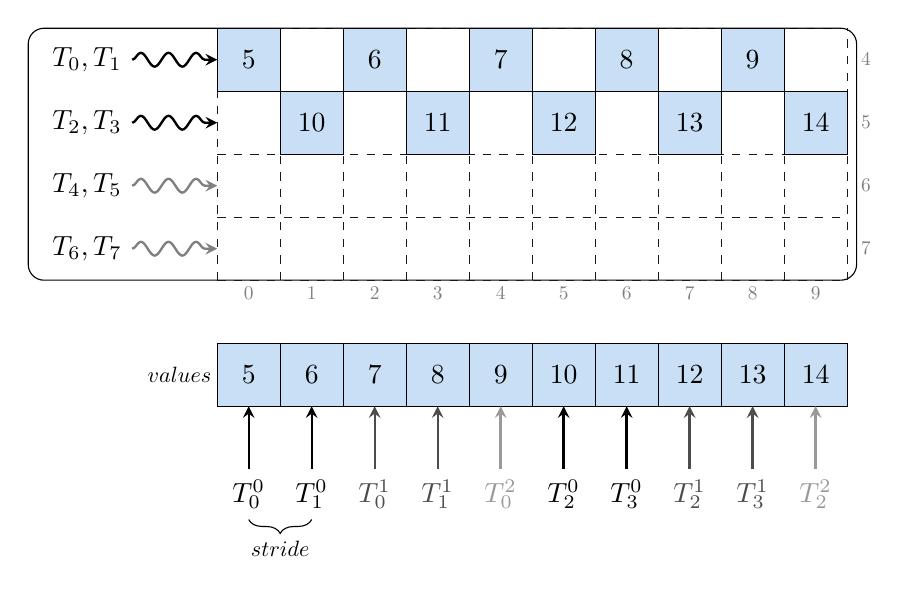
\begin{tikzpicture}[circ/.style = {circle, draw, inner sep=0pt, minimum size=3pt, outer sep=0pt, minimum size=6mm}, scale=0.8]

  \draw[round] (-3.0,2.0) rectangle (10.15,6.0);

	\draw[draw=black,snake it,line width=0.30mm,>=stealth,->]   (-1.35,5.5) node [anchor=east] {$T_0,T_1$} -- (0,5.5);
	\draw[draw=black,snake it,line width=0.30mm,>=stealth,->]   (-1.35,4.5) node [anchor=east] {$T_2,T_3$} -- (0,4.5);
	\draw[draw=gray,snake it,line width=0.30mm,>=stealth,->] (-1.35,3.5) node [anchor=east] {$T_4,T_5$} -- (0,3.5);
	\draw[draw=gray,snake it,line width=0.30mm,>=stealth,->] (-1.35,2.5) node [anchor=east] {$T_6,T_7$} -- (0,2.5);

  \foreach \y in {4,...,7} {
    \node[scale=0.7,text=gray] at (10.3,10.0 - 1.0*\y - 0.5) {\y};
  }

  \foreach \x in {0,...,9} {
    \node[scale=0.7,text=gray] at (1.0*\x + 0.5,1.8) {\x};
  }

  % Elements mesh
  \draw[step=1.0,black!90!white,thin,dashed,line width=0.4] (0.0,2.0) grid (10.0,6.0);

  \edef\esize{1.0}

  % ROW 0
  \edef\elementnum{5}

  % ROW 4
  \foreach \col in {0,2,4,6,8} {
    \draw[fill=r1d!60] (\col*\esize,5.0) rectangle (\col*\esize+\esize,6) node[pos=.5] {\elementnum};
    \pgfmathparse{int(\elementnum+1)}
    \xdef\elementnum{\pgfmathresult}
  }

  % ROW 5
  \foreach \col in {1,3,5,7,9} {
    \draw[fill=r1d!60] (\col*\esize,4.0) rectangle (\col*\esize+\esize,5) node[pos=.5] {\elementnum};
    \pgfmathparse{int(\elementnum+1)}
    \xdef\elementnum{\pgfmathresult}
  }

  % Data access
  \pgfmathparse{2-\esize*2}
  \xdef\ybot{\pgfmathresult}

  \node[scale=0.8] at (-0.6,\ybot+\esize/2) {$values$};

  % Row 0
  \edef\elementnum{5}

  % Row 4
  \foreach \i in {0,...,4} {
    \draw[fill=r1d!60]  (\i * \esize,\ybot) rectangle (\i * \esize + \esize,\ybot+\esize) node[pos=0.5] {\elementnum};
    \pgfmathparse{int(\elementnum+1)}
    \xdef\elementnum{\pgfmathresult}
  }

	\draw[draw=black!100,line width=0.30mm,>=stealth,->] (\esize/2,\ybot-\esize) node [anchor=north] {$T_0^0$} -- (\esize/2,\ybot);
	\draw[draw=black!100,line width=0.30mm,>=stealth,->] (\esize+\esize/2,\ybot-\esize) node [anchor=north] {$T_1^0$} -- (\esize+\esize/2,\ybot);
	\draw[draw=black!70,text=black!70,line width=0.30mm,>=stealth,->] (2*\esize+\esize/2,\ybot-\esize) node [anchor=north] {$T_0^1$} -- (2*\esize+\esize/2,\ybot);
	\draw[draw=black!70,text=black!70,line width=0.30mm,>=stealth,->] (3*\esize+\esize/2,\ybot-\esize) node [anchor=north] {$T_1^1$} -- (3*\esize+\esize/2,\ybot);
	\draw[draw=black!40,text=black!40,line width=0.30mm,>=stealth,->] (4*\esize+\esize/2,\ybot-\esize) node [anchor=north] {$T_0^2$} -- (4*\esize+\esize/2,\ybot);

  % Row 5
  \foreach \i in {5,...,9} {
    \draw[fill=r1d!60]  (\i * \esize,\ybot) rectangle (\i * \esize + \esize,\ybot+\esize) node[pos=0.5] {\elementnum};
    \pgfmathparse{int(\elementnum+1)}
    \xdef\elementnum{\pgfmathresult}
  }

	\draw[draw=black!100,line width=0.30mm,>=stealth,->] (5*\esize+\esize/2,\ybot-\esize) node [anchor=north] {$T_2^0$} -- (5*\esize+\esize/2,\ybot);
	\draw[draw=black!100,line width=0.30mm,>=stealth,->]  (6*\esize+\esize/2,\ybot-\esize) node [anchor=north] {$T_3^0$} -- (6*\esize+\esize/2,\ybot);
	\draw[draw=black!70,text=black!70,line width=0.30mm,>=stealth,->]  (7*\esize+\esize/2,\ybot-\esize) node [anchor=north] {$T_2^1$} -- (7*\esize+\esize/2,\ybot);
	\draw[draw=black!70,text=black!70,line width=0.30mm,>=stealth,->]  (8*\esize+\esize/2,\ybot-\esize) node [anchor=north] {$T_3^1$} -- (8*\esize+\esize/2,\ybot);
	\draw[draw=black!40,text=black!40,line width=0.30mm,>=stealth,->]  (9*\esize+\esize/2,\ybot-\esize) node [anchor=north] {$T_2^2$} -- (9*\esize+\esize/2,\ybot);

  \draw [mbrace] (\esize/2,\ybot-1.8*\esize) -- (1*\esize+\esize/2,\ybot-1.8*\esize) node[bottomlabel] {$stride$};

  \end{tikzpicture}
  \caption{CSR-Scalar block's threads' work distribution}
  \label{csr_vector_format_mem_access_pattern}
\end{figure}

In the case of CSR-Vector reduction might be implemented using warp-level primitives (list. \ref{warp_reduce}). In that case, the data 
exchange is performed between registers and more efficient than going through shared memory, which requires a load, 
a store, and an extra register to hold the address.

\begin{listing}[H]
\begin{minted}[linenos,tabsize=2]{cuda}
template <class T>
__device__ T warp_reduce (T val)
{
  for (int offset = warpSize / 2; offset > 0; offset /= 2)
    val += __shfl_down_sync (FULL_WARP_MASK, val, offset);

  return val;
}
\end{minted}
\caption{Warp reduction}
\label{warp_reduce}
\end{listing}

\begin{listing}[H]
\begin{minted}[linenos,tabsize=2]{cuda}
template <typename data_type>
__global__ void csr_spmv_vector_kernel (
    unsigned int n_rows,
    const unsigned int *col_ids,
    const unsigned int *row_ptr,
    const data_type *data,
    const data_type *x,
    data_type *y)
{
  const unsigned int thread_id = blockIdx.x * blockDim.x + threadIdx.x;
  const unsigned int warp_id = thread_id / 32;
  const unsigned int lane = thread_id % 32;

  const unsigned int row = warp_id; ///< One warp per row

  data_type sum = 0;
  if (row < n_rows)
  {
    const unsigned int row_start = row_ptr[row];
    const unsigned int row_end = row_ptr[row + 1];

    for (unsigned int element = row_start + lane; element < row_end; element += 32)
      sum += data[element] * x[col_ids[element]];
  }

  sum = warp_reduce (sum);

  if (lane == 0 && row < n_rows)
    y[row] = sum;
}
\end{minted}
\caption{SpMV kernel for the CSR sparse matrix format (vector)}
\label{csr_vector}
\end{listing}

CSR-Vector has better speedup (tab. \ref{csr_vector_speedup_table}) and speedup distribution (fig. \ref{csr_vector_speedup_float} and \ref{csr_vector_speedup_double}) 
than CSR-Scalar (for both float and double matrices) and cuSPARSE implementation (for float matrices). 

\begin{table}[H]
	\centering
	\begin{tabular}{ |p{2.6cm}||p{1cm}|p{1cm}|p{1cm}|p{1cm}|  }
	 \hline
		& \multicolumn{2}{|c|}{float} & \multicolumn{2}{|c|}{double}\\
	 \hline
	 NNZ lower limit & avg & max & avg & max  \\
	 \hline
	 10000  & 6.60  & 43.46 & 4.37 & 29.62 \\
	 100000 & 14.40 & 43.46 & 9.50 & 29.62 \\
	 \hline
	\end{tabular}
	\caption{CSR-Vector speedup}
  \label{csr_vector_speedup_table}
\end{table}

\begin{figure}[H]
\centering
\subfloat[CSR-Vector speedup (float) \label{csr_vector_speedup_float}]  {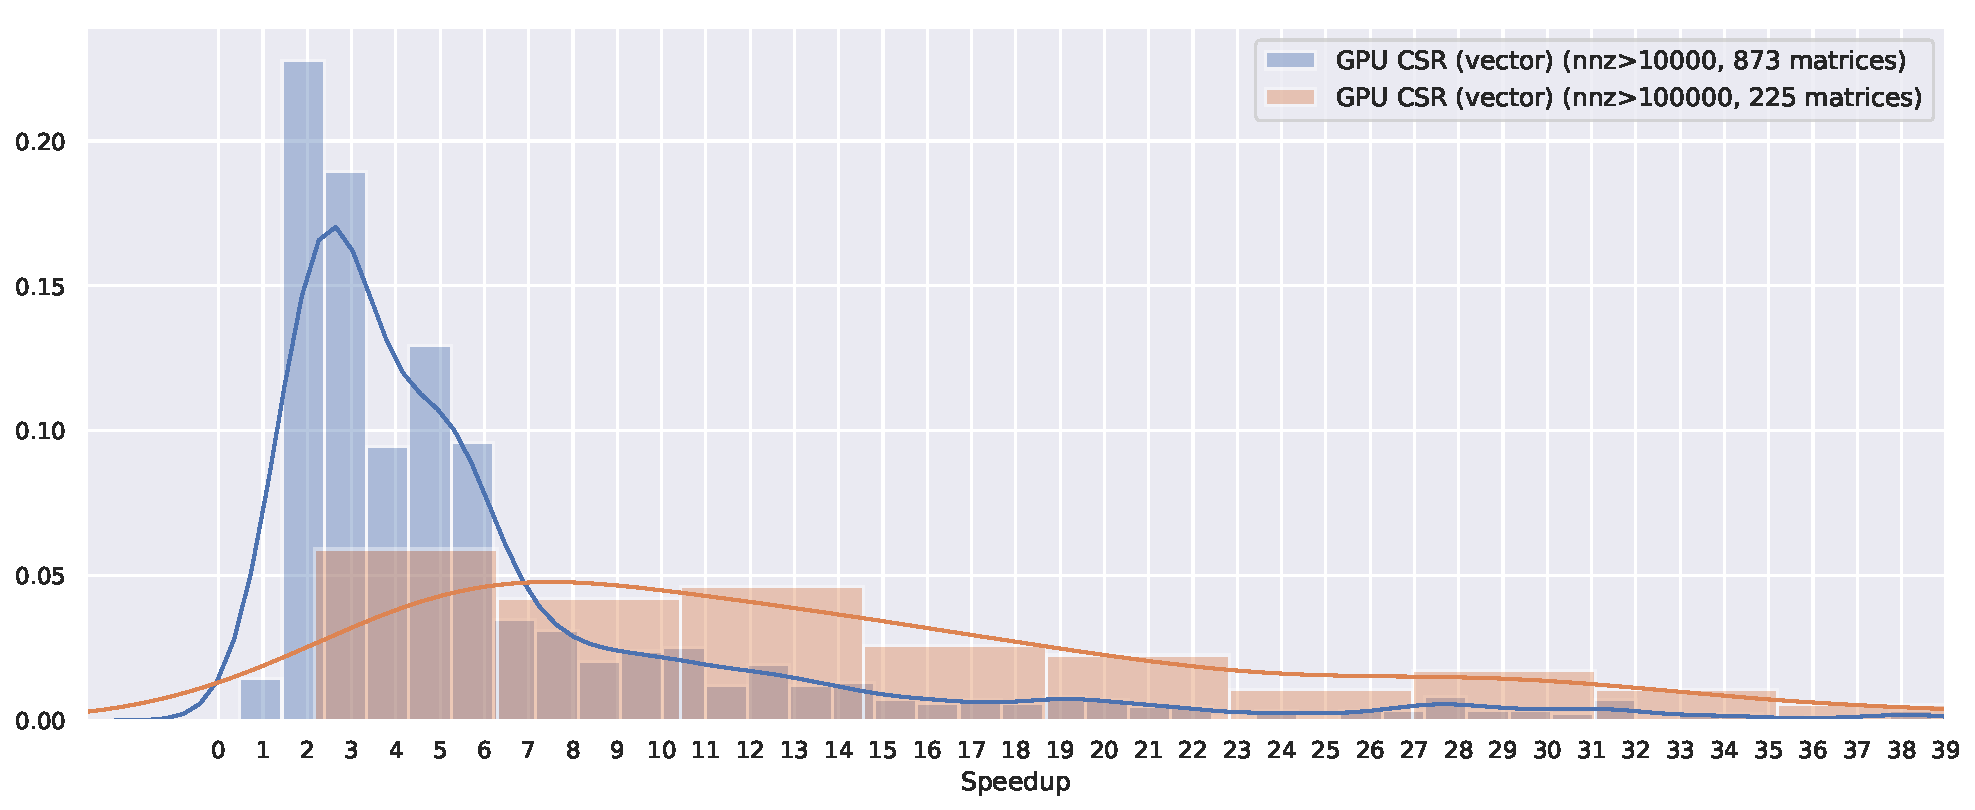
\includegraphics[width=1.0\textwidth]{img/csr_vector_float_dist.pdf}}
\qquad %
\subfloat[CSR-Vector speedup (double) \label{csr_vector_speedup_double}] {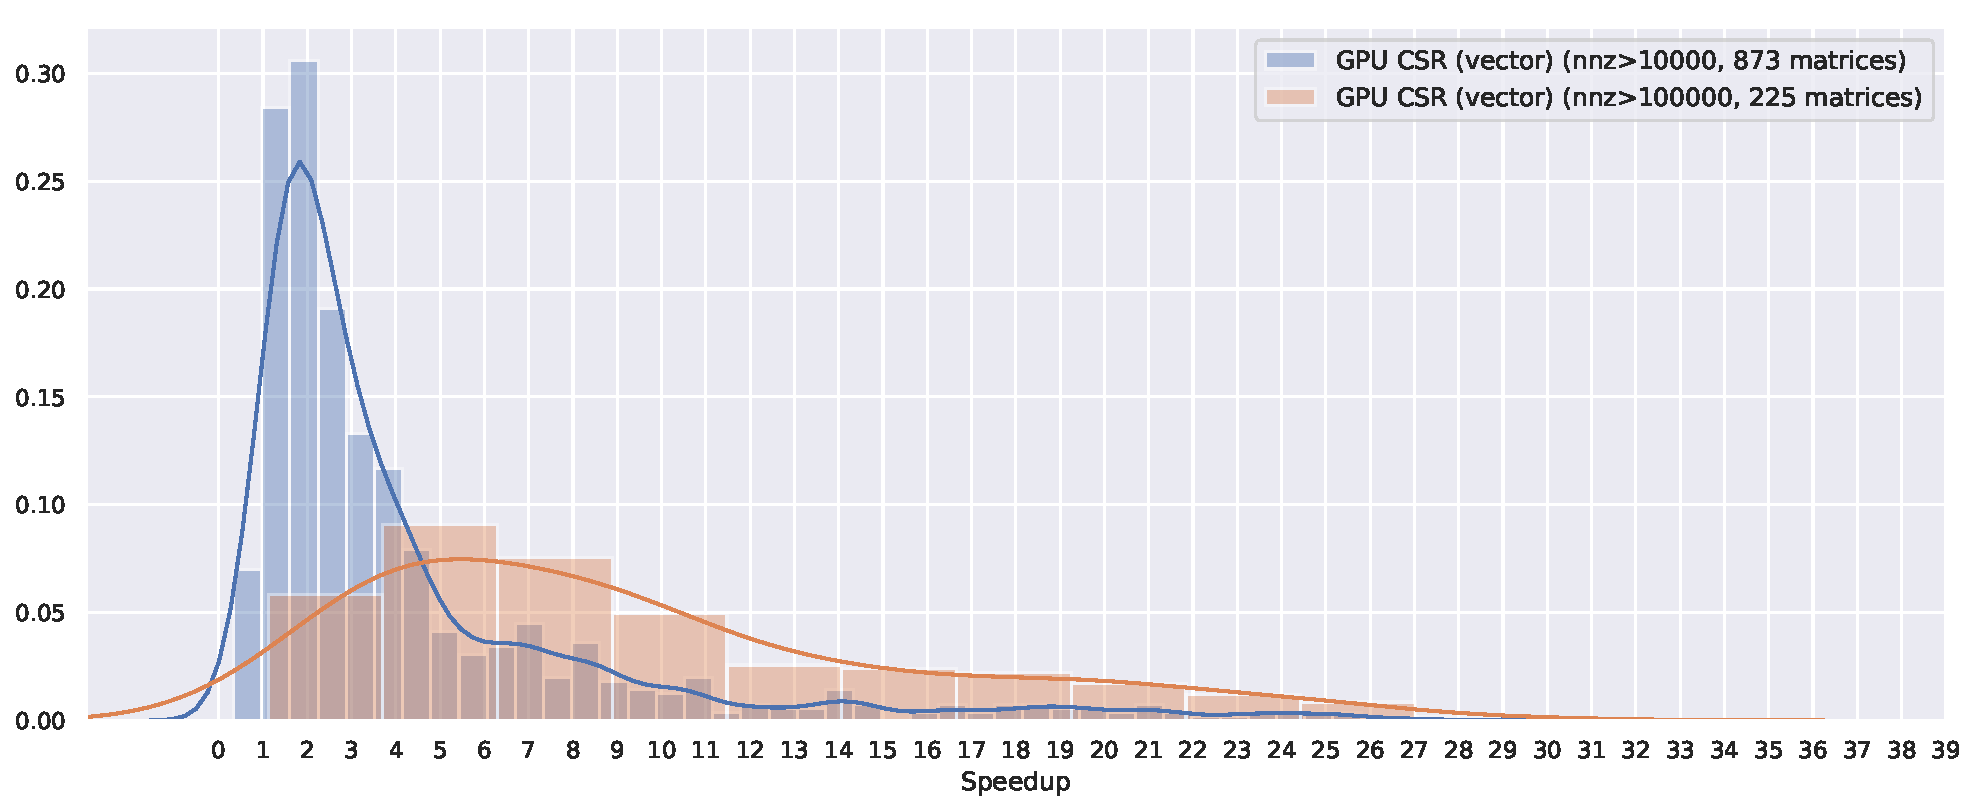
\includegraphics[width=1.0\textwidth]{img/csr_vector_double_dist.pdf}}
\end{figure}

However, CSR-Scalar outperforms CSR-Vector on about $33\%$ of float matrices with $10000$ nnz lower limit and on $40\%$ of float matrices with $100000$ nnz lower limit 
(fig \ref{csr_csr_outperform_vec} and \ref{vec_csr_outperform_vec}). On that matrices, CSR shows average speedup equal to $8.57$ while CSR-Vector
only $4.80$. 

\begin{figure}[H]
\centering
\subfloat[CSR-Vector speedup (float) \label{csr_csr_outperform_vec}]  {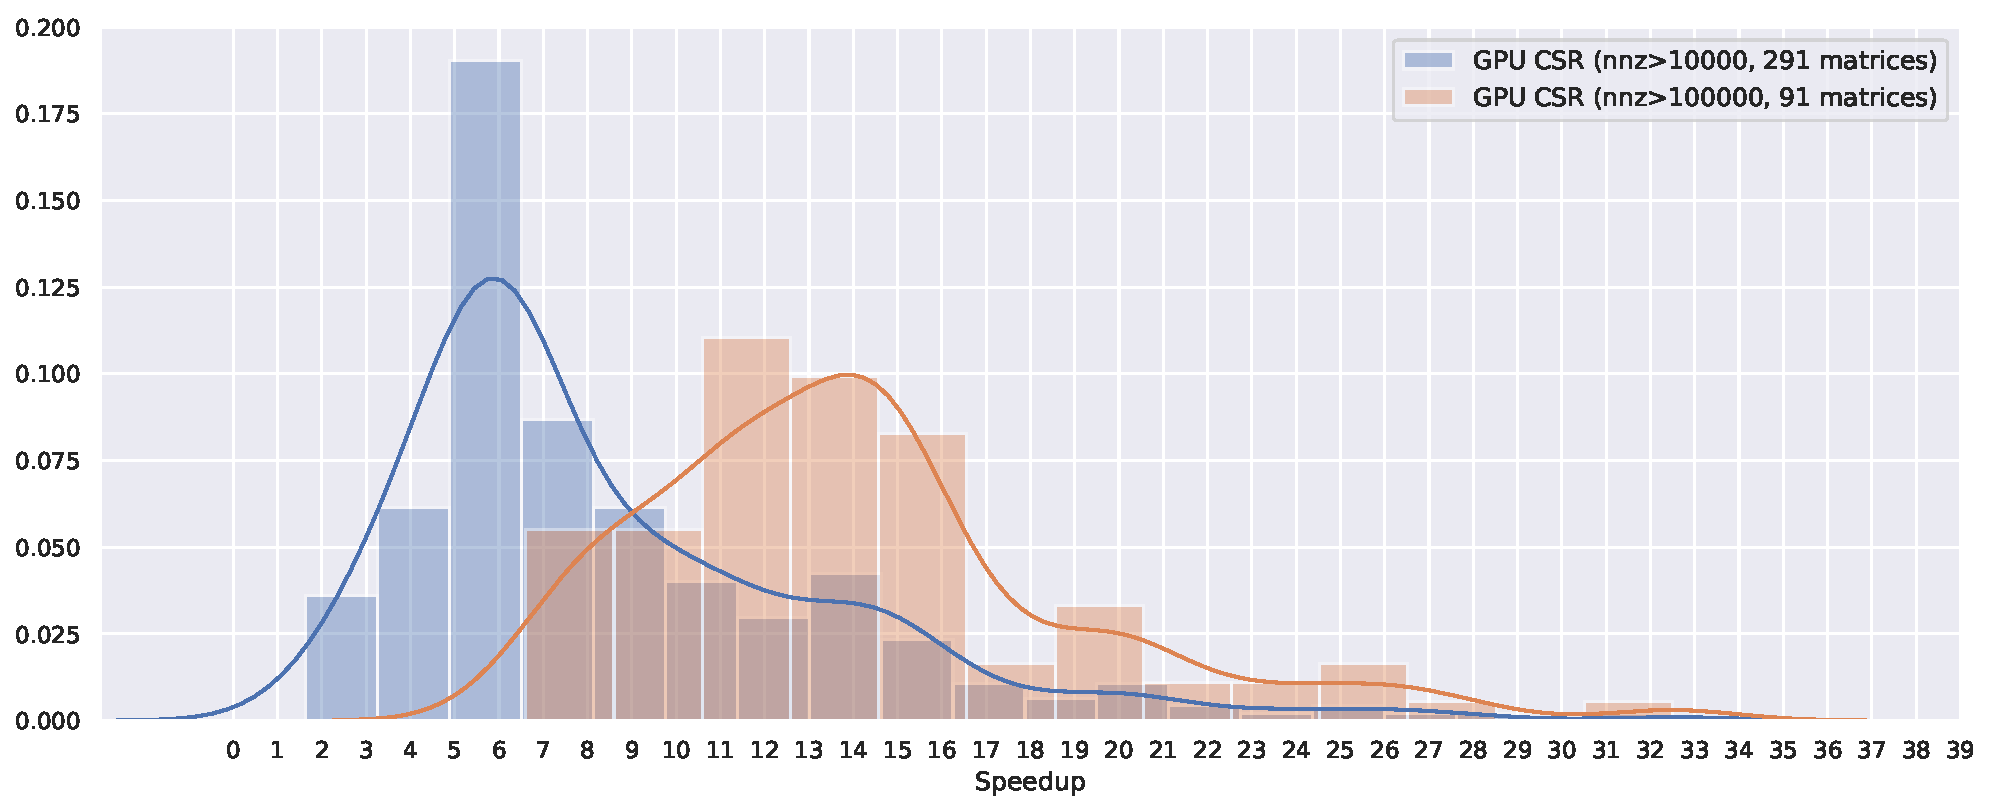
\includegraphics[width=1.0\textwidth]{img/csr_csr_outperform_csr_vec.pdf}}
\qquad %
\subfloat[CSR-Vector speedup (double) \label{vec_csr_outperform_vec}] {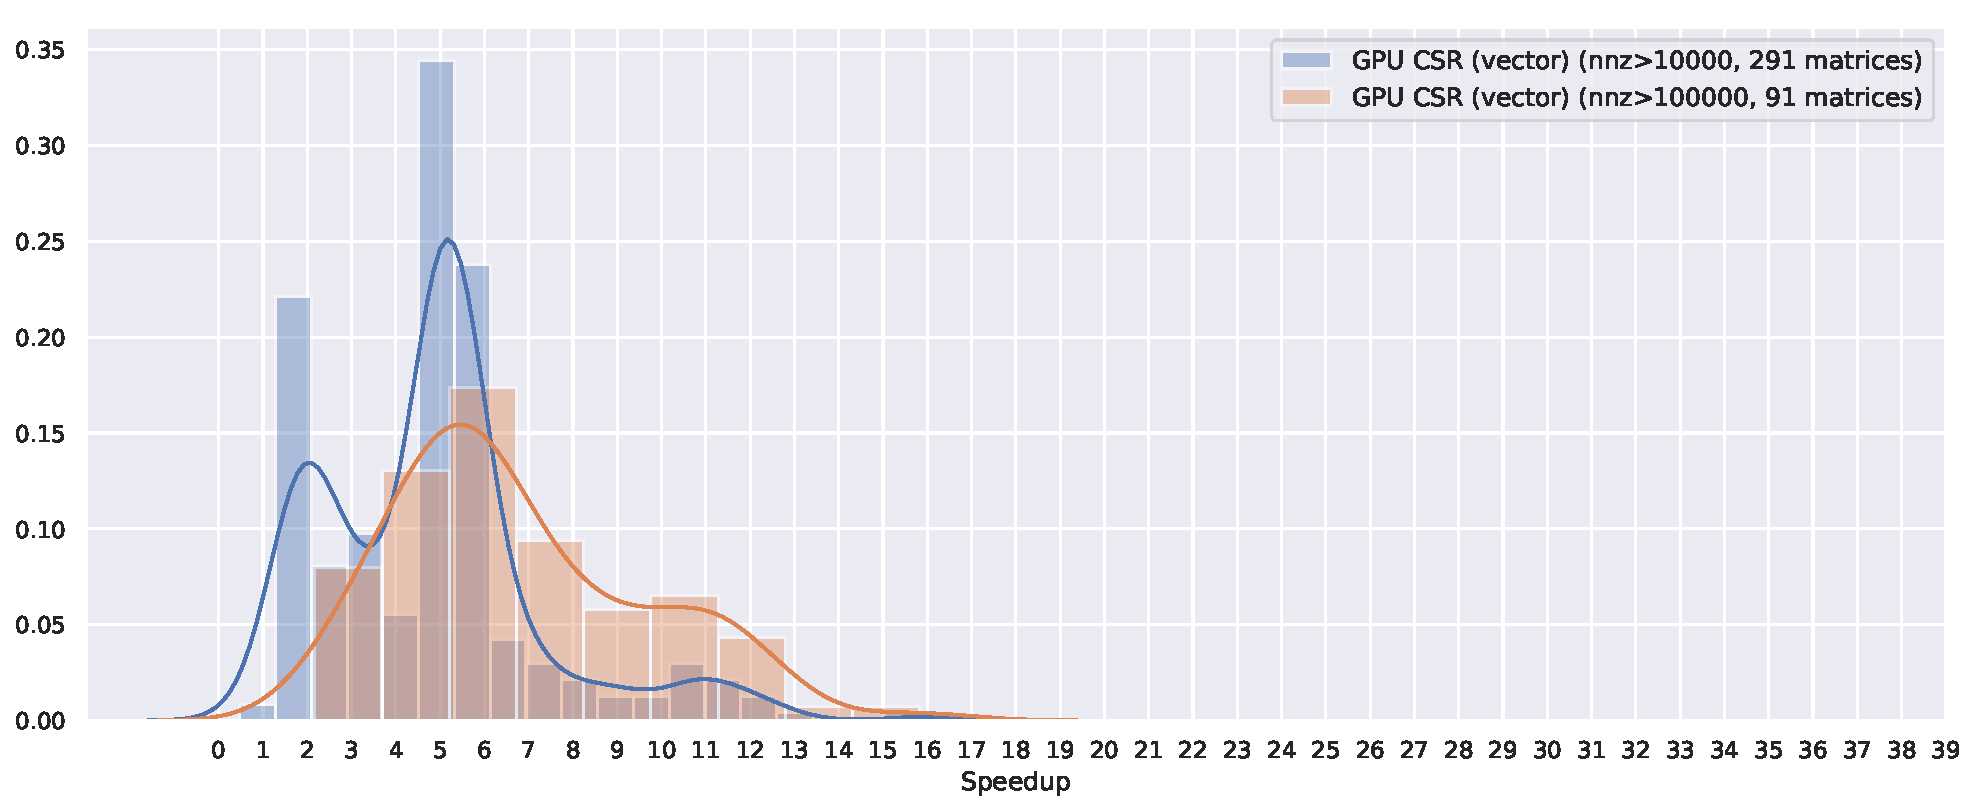
\includegraphics[width=1.0\textwidth]{img/vec_csr_outperform_csr_vec.pdf}}
\end{figure}

To discover further improvements of CSR SpMV implementation, we need to consider the first matrix part from figure \ref{csr_format}. In the first four rows
of the matrix, there is only one non-zero value per row. In that case whole warp's threads except first are idle. In this case, it's possible
for naive CSR SpMV implementation to outperform vector implementation. There is an SpMV algorithm for the CSR matrix format that doesn't depend on nnz/row ratio.
The CSR-Adaptive changes it's behavior depending on the nnz in each row (list. \ref{csr_adaptive}). After selecting non-zeroes per block value,
additional array ($row\_blocks$) for storing block rows is constructed. If some rows contain small nnz, they'll be gathered into one block. Then
CUDA threads block is assigned to each rows block. The case of multiple rows in one rows block is called CSR-Stream. If there is only one row
in rows block, the CSR-Vector will be called. If this row exceeds $nnz\_per\_wg$ than CSR-VectorL variant will be used. The main difference between
CSR-Vector and CSR-VectorL is that CSR-VectorL allows executing multiple CSR-VectorL on one row and then reducing the results by using atomic operations.

\begin{listing}[H]
\begin{minted}[linenos,tabsize=2]{cuda}
template <typename data_type>
__global__ void csr_adaptive_spmv_kernel (
    const unsigned int n_rows,
    const unsigned int *col_ids,
    const unsigned int *row_ptr,
    const unsigned int *row_blocks,
    const data_type *data,
    const data_type *x,
    data_type *y)
{
  const unsigned int block_row_begin = row_blocks[blockIdx.x];
  const unsigned int block_row_end = row_blocks[blockIdx.x + 1];

  __shared__ data_type cache[NNZ_PER_WG];

  if (block_row_end - block_row_begin > 1)
  {
    /// CSR-Stream case...
\end{minted}
\begin{minted}[linenos,tabsize=2,firstnumber=94]{cuda}
  }
  else
  {
    const unsigned int nnz = row_ptr[block_row_end] - row_ptr[block_row_begin];

    if (nnz <= 64)
    {
      /// CSR-Vector case...
\end{minted}
\begin{minted}[linenos,tabsize=2,firstnumber=118]{cuda}
    }
    else
    {
      /// CSR-VectorL case...
\end{minted}
\begin{minted}[linenos,tabsize=2,firstnumber=151]{cuda}
    }
  }
}
\end{minted}
\caption{SpMV kernel for the CSR-Adaptive sparse matrix format}
\label{csr_adaptive}
\end{listing}


The CSR-Vector and CSR-VectorL parts are quite similar CSR-Vector algorithm, so I won't include listing here. Figure \ref{csr_adaptive_format_mem_access_pattern}
illustrates memory access pattern of the CSR-Stream part. It stores partial sums in shared memory of GPU and then reduces them. The partial results in cache in
figure \ref{csr_adaptive_format_mem_access_pattern} are calculated with $x$ filled with $1$. The source code of CSR-Stream is presented in listing \ref{csr_stream_implementation}.

\begin{figure}[H]
  \centering
  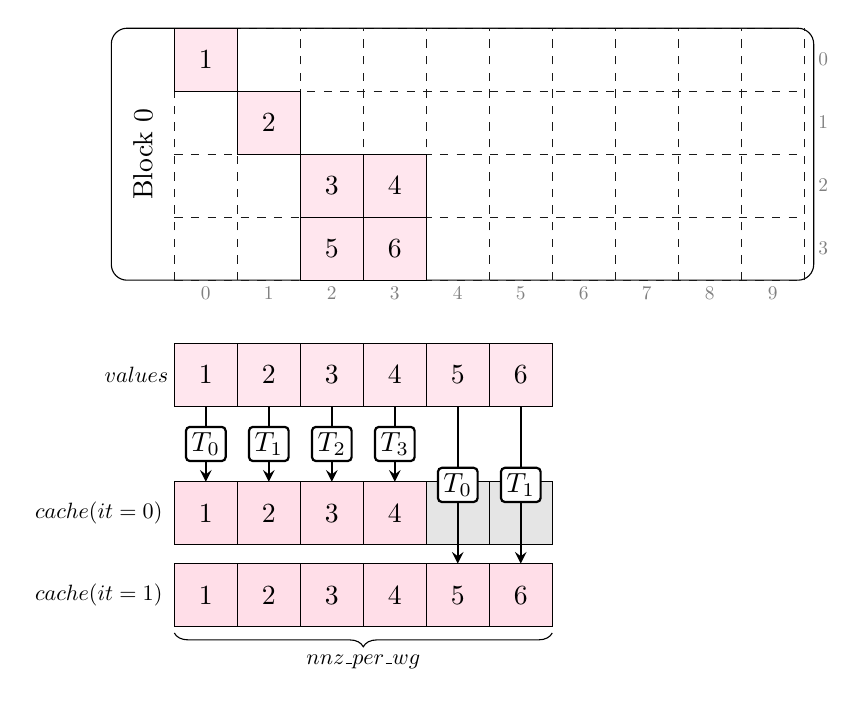
\begin{tikzpicture}[circ/.style = {circle, draw, inner sep=0pt, minimum size=3pt, outer sep=0pt, minimum size=6mm}, scale=0.8]

  \draw[round] (-1.0,2.0) rectangle (10.15,6.0);
  \node[rotate=90] at (-0.5,4) {Block 0};

  \foreach \y in {0,...,3} {
    \node[scale=0.7,text=gray] at (10.3,10.0 - 1.0*\y - 4.5) {\y};
  }

  \foreach \x in {0,...,9} {
    \node[scale=0.7,text=gray] at (1.0*\x + 0.5,1.8) {\x};
  }

  % Elements mesh
  \draw[step=1.0,black!90!white,thin,dashed,line width=0.4] (0.0,2.0) grid (10.0,6.0);

  \edef\esize{1.0}

  % ROW 0
  \edef\elementnum{1}
  \foreach \col in {0} {
    \draw[fill=r0d!60] (\col*\esize,5.0) rectangle (\col*\esize+\esize,6) node[pos=.5] {\elementnum};
    \pgfmathparse{int(\elementnum+1)}
    \xdef\elementnum{\pgfmathresult}
  }

  \foreach \col in {1} {
    \draw[fill=r0d!60] (\col*\esize,4.0) rectangle (\col*\esize+\esize,5) node[pos=.5] {\elementnum};
    \pgfmathparse{int(\elementnum+1)}
    \xdef\elementnum{\pgfmathresult}
  }

  \foreach \col in {2,3} {
    \draw[fill=r0d!60] (\col*\esize,3.0) rectangle (\col*\esize+\esize,4) node[pos=.5] {\elementnum};
    \pgfmathparse{int(\elementnum+1)}
    \xdef\elementnum{\pgfmathresult}
  }

  \foreach \col in {2,3} {
    \draw[fill=r0d!60] (\col*\esize,2.0) rectangle (\col*\esize+\esize,3) node[pos=.5] {\elementnum};
    \pgfmathparse{int(\elementnum+1)}
    \xdef\elementnum{\pgfmathresult}
  }


  % Data access
  \pgfmathparse{2-\esize*2}
  \xdef\ybot{\pgfmathresult}

  \node[scale=0.8] at (-0.6,\ybot+\esize/2) {$values$};

  \edef\elementnum{1}
  \foreach \i in {0,...,5} {
    \draw[fill=r0d!60]  (\i * \esize,\ybot) rectangle (\i * \esize + \esize,\ybot+\esize) node[pos=0.5] {\elementnum};
    \pgfmathparse{int(\elementnum+1)}
    \xdef\elementnum{\pgfmathresult}
  }

	\draw[draw=black,line width=0.30mm,>=stealth,->] (\esize/2,\ybot) -- (\esize/2,\ybot-1.2*\esize) node [midway,draw=black,fill=white,thick,rounded corners=.05cm,inner sep=2pt] {$T_0$};
	\draw[draw=black,line width=0.30mm,>=stealth,->] (\esize+\esize/2,\ybot) -- (\esize+\esize/2,\ybot-1.2*\esize) node [midway,draw=black,fill=white,thick,rounded corners=.05cm,inner sep=2pt] {$T_1$};
	\draw[draw=black,line width=0.30mm,>=stealth,->] (2*\esize+\esize/2,\ybot) -- (2*\esize+\esize/2,\ybot-1.2*\esize) node [midway,draw=black,fill=white,thick,rounded corners=.05cm,inner sep=2pt] {$T_2$};
	\draw[draw=black,line width=0.30mm,>=stealth,->] (3*\esize+\esize/2,\ybot) -- (3*\esize+\esize/2,\ybot-1.2*\esize) node [midway,draw=black,fill=white,thick,rounded corners=.05cm,inner sep=2pt] {$T_3$};

  \pgfmathparse{\ybot-2.2*\esize}
  \xdef\ybot{\pgfmathresult}

  \edef\elementnum{1}
  \foreach \i in {0,...,3} {
    \draw[fill=r0d!80]  (\i * \esize,\ybot) rectangle (\i * \esize + \esize,\ybot+\esize) node[pos=0.5] {\elementnum};
    \pgfmathparse{int(\elementnum+1)}
    \xdef\elementnum{\pgfmathresult}
  }
  \foreach \i in {4,...,5} {
    \draw[fill=gray!20]  (\i * \esize,\ybot) rectangle (\i * \esize + \esize,\ybot+\esize) node[pos=0.5] {};
    \pgfmathparse{int(\elementnum+1)}
    \xdef\elementnum{\pgfmathresult}
  }

  \node[scale=0.8] at (-1.2,\ybot+\esize/2) {$cache(it=0)$};

  \pgfmathparse{\ybot-1.3*\esize}
  \xdef\ybot{\pgfmathresult}
  \node[scale=0.8] at (-1.2,\ybot+\esize/2) {$cache(it=1)$};

  \edef\elementnum{1}
  \foreach \i in {0,...,5} {
    \draw[fill=r0d!80]  (\i * \esize,\ybot) rectangle (\i * \esize + \esize,\ybot+\esize) node[pos=0.5] {\elementnum};
    \pgfmathparse{int(\elementnum+1)}
    \xdef\elementnum{\pgfmathresult}
  }

  \draw [mbrace] (0,\ybot-0.1) -- (6*\esize,\ybot-0.1) node[bottomlabel] {$nnz\_per\_wg$};

	\draw[draw=black,line width=0.30mm,>=stealth,->] (4*\esize+\esize/2,\ybot+3.5) -- (4*\esize+\esize/2,\ybot+\esize) node [midway,draw=black,fill=white,thick,rounded corners=.05cm,inner sep=2pt] {$T_0$};
	\draw[draw=black,line width=0.30mm,>=stealth,->] (5*\esize+\esize/2,\ybot+3.5) -- (5*\esize+\esize/2,\ybot+\esize) node [midway,draw=black,fill=white,thick,rounded corners=.05cm,inner sep=2pt] {$T_1$};

  \end{tikzpicture}
  \caption{CSR-Stream memory access pattern}
  \label{csr_adaptive_format_mem_access_pattern}
\end{figure}

\begin{listing}[H]
\begin{minted}[linenos,tabsize=2,firstnumber=19,fontsize=\footnotesize]{cuda}
const unsigned int i = threadIdx.x;
const unsigned int block_data_begin = row_ptr[block_row_begin];
const unsigned int thread_data_begin = block_data_begin + i;

if (i < nnz)
	cache[i] = data[thread_data_begin] * x[col_ids[thread_data_begin]];
__syncthreads ();

const unsigned int threads_for_reduction = prev_power_of_2 (blockDim.x / (block_row_end - block_row_begin));

if (threads_for_reduction > 1)
	{
		/// Reduce all non zeroes of row by multiple thread
		const unsigned int thread_in_block = i % threads_for_reduction;
		const unsigned int local_row = block_row_begin + i / threads_for_reduction;

		data_type sum = 0.0;

		if (local_row < block_row_end)
			{
				const unsigned int local_first_element = row_ptr[local_row] - row_ptr[block_row_begin];
				const unsigned int local_last_element = row_ptr[local_row + 1] - row_ptr[block_row_begin];

				for (unsigned int local_element = local_first_element + thread_in_block;
						 local_element < local_last_element;
						 local_element += threads_for_reduction)
					{
						sum += cache[local_element];
					}
			}
		__syncthreads ();
		cache[i] = sum;

		/// Now each row has threads_for_reduction values in cache
		for (int j = threads_for_reduction / 2; j > 0; j /= 2)
			{
				/// Reduce for each row
				__syncthreads ();

				const bool use_result = thread_in_block < j && i + j < NNZ_PER_WG;

				if (use_result)
					sum += cache[i + j];
				__syncthreads ();

				if (use_result)
					cache[i] = sum;
			}

		if (thread_in_block == 0 && local_row < block_row_end)
			y[local_row] = sum;
	}
else
	{
		/// Reduce all non zeroes of row by single thread
		unsigned int local_row = block_row_begin + i;
		while (local_row < block_row_end)
			{
				data_type sum = 0.0;

				for (unsigned int j = row_ptr[local_row] - block_data_begin;
						 j < row_ptr[local_row + 1] - block_data_begin;
						 j++)
					{
						sum += cache[j];
					}

				y[local_row] = sum;
				local_row += NNZ_PER_WG;
			}
	}
\end{minted}
\caption{CSR-Stream implementation}
\label{csr_stream_implementation}
\end{listing}

On the discussed set of matrices (fig. \ref{csr_csr_outperform_vec} and \ref{vec_csr_outperform_vec}), where CSR outperformed CSR-Vector, CSR-Adaptive
shows better speedup. CSR-Adaptive outperforms CSR-Scalar on those $291$ matrices.
Although CSR-Adaptive might be outperformed by CSR-Vector on some long-row matrices, it has better speedup in average (tab. \ref{csr_vector_speedup_table}, 
fig. \ref{csr_adaptive_speedup_float} and \ref{csr_adaptive_speedup_double}). The main advantage of CSR-Adaptive is that you won't need to change
the code that generates a matrix if your code already uses CSR. The matrix formats presented below don't have this quality.

\begin{table}[H]
	\centering
	\begin{tabular}{ |p{2.6cm}||p{1cm}|p{1cm}|p{1cm}|p{1cm}|  }
	 \hline
		& \multicolumn{2}{|c|}{float} & \multicolumn{2}{|c|}{double}\\
	 \hline
	 NNZ lower limit & avg & max & avg & max  \\
	 \hline
	 10000  & 7.37  & 48.19 & 6.39 & 40.39 \\
	 100000 & 14.27 & 48.19 & 11.72 & 40.39 \\
	 \hline
	\end{tabular}
	\caption{CSR-Adaptive speedup}
  \label{csr_vector_speedup_table}
\end{table}

\begin{figure}[H]
\centering
\subfloat[CSR-Adaptive speedup (float) \label{csr_adaptive_speedup_float}]  {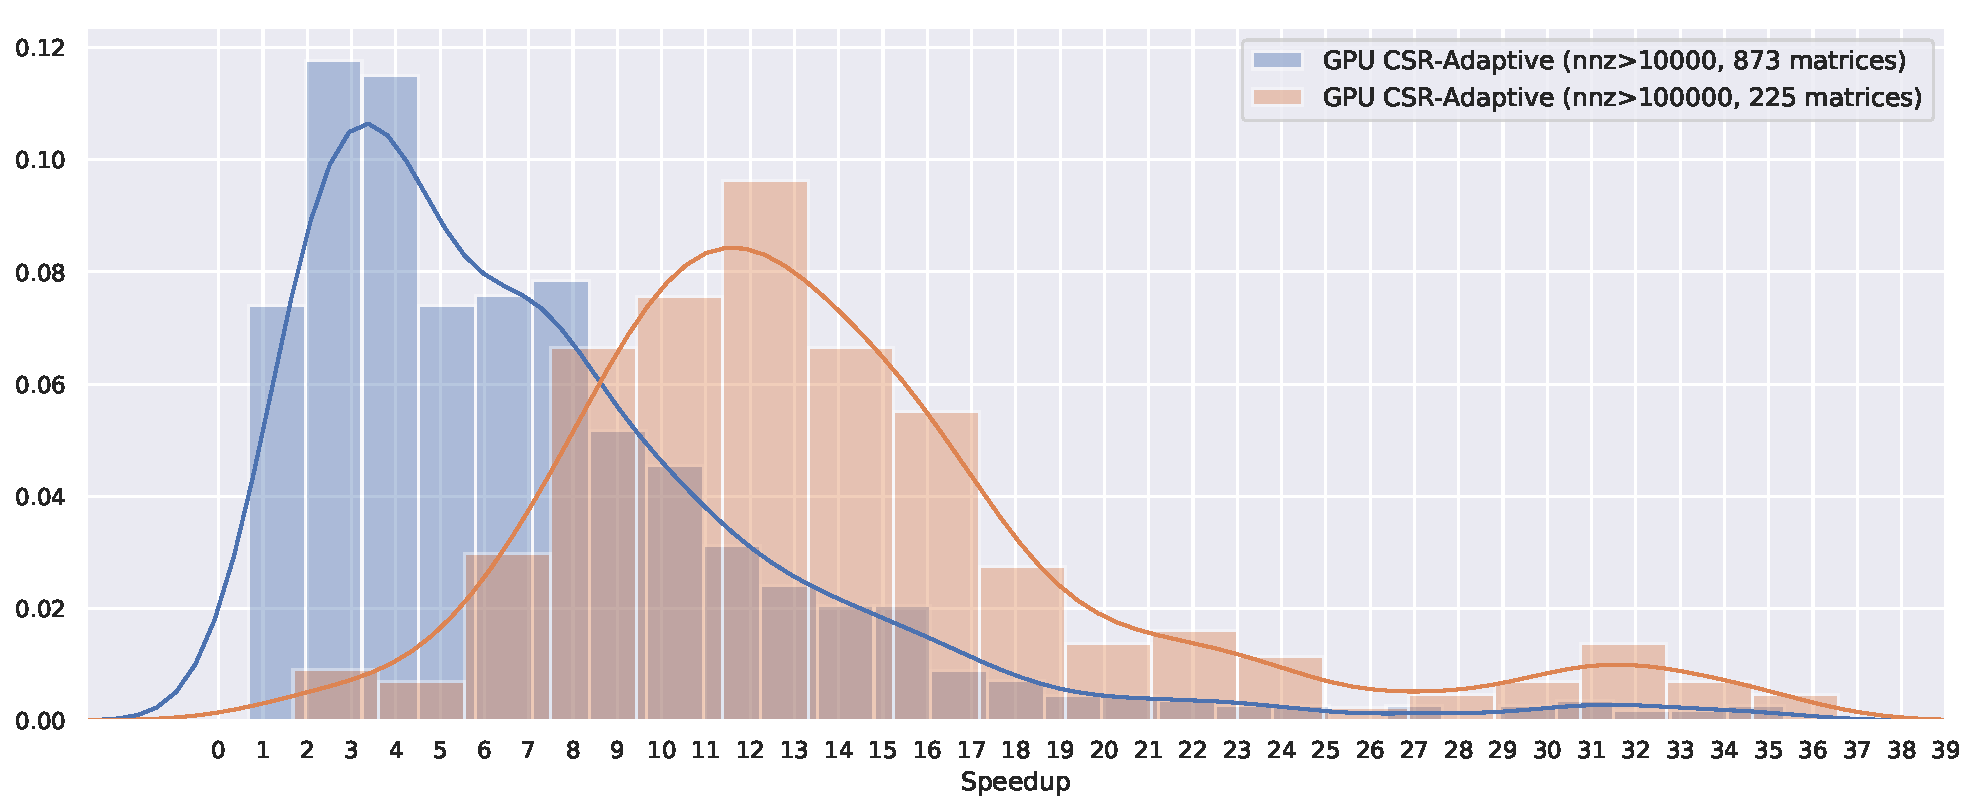
\includegraphics[width=1.0\textwidth]{img/csr_adaptive_float_dist.pdf}}
\qquad %
\subfloat[CSR-Adaptive speedup (double) \label{csr_adaptive_speedup_double}] {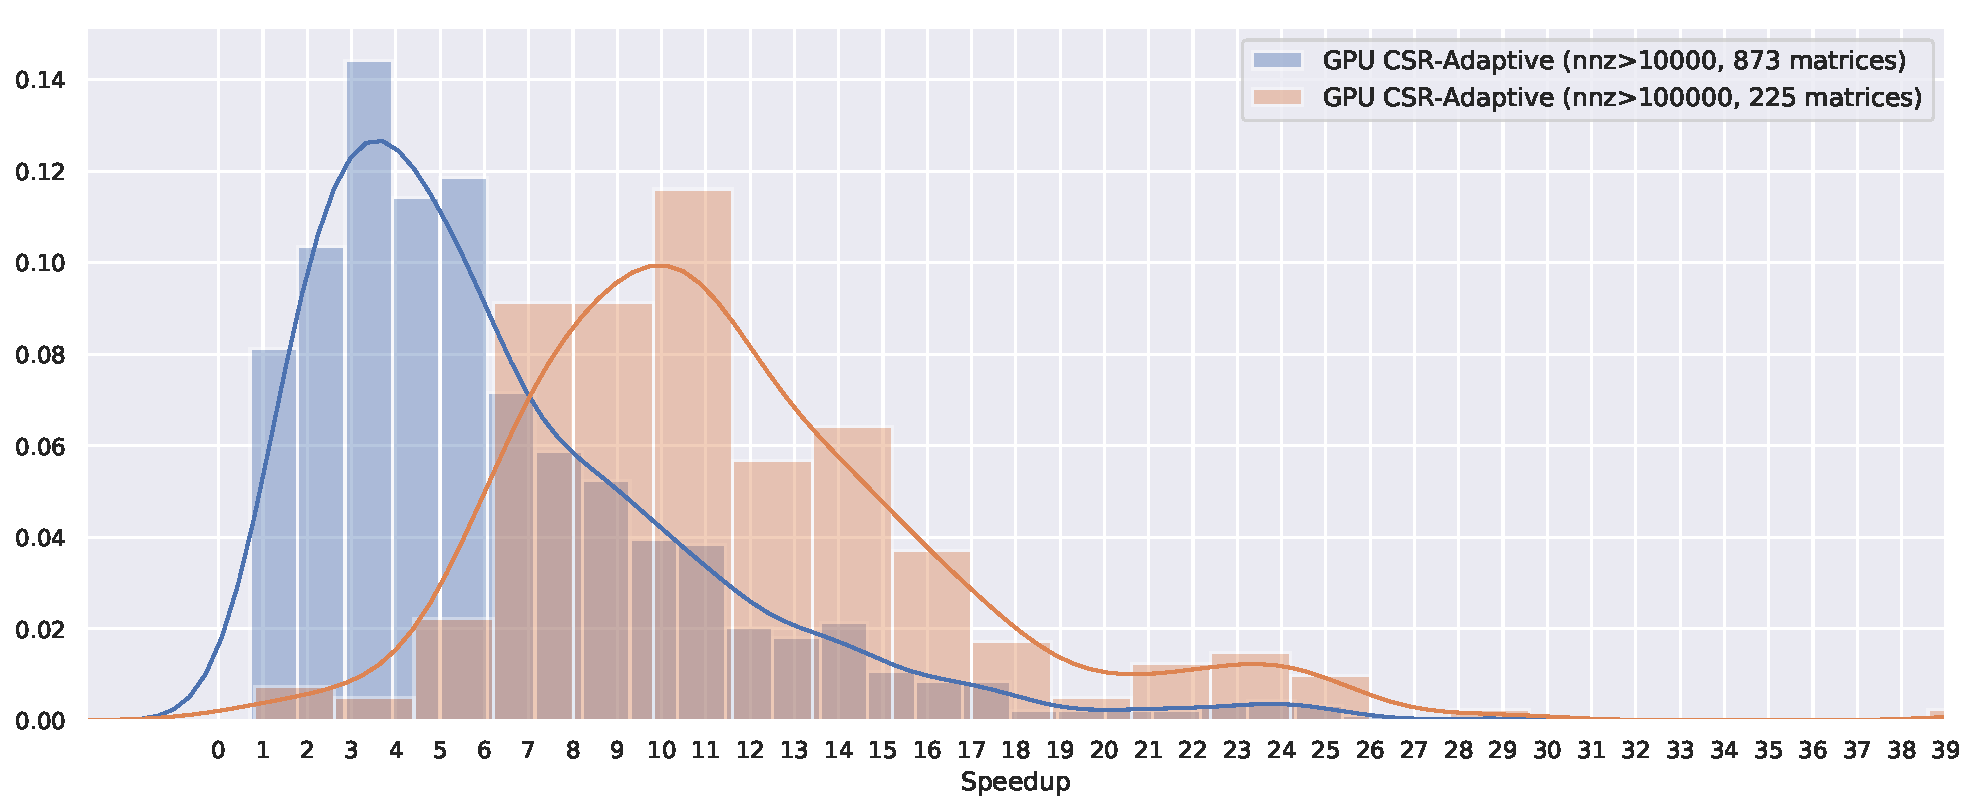
\includegraphics[width=1.0\textwidth]{img/csr_adaptive_double_dist.pdf}}
\end{figure}




\subsection{ELL}
The problem of noncoalesced memory accesses of CSR can be addressed by applying data padding and transposition on the sparse matrix data (fig. \ref{ell_format}).
The Ellpack-Itpack (ELL) sparse matrix format assumes that each row contains at most \textit{elements\_in\_rows} elements and \textit{elements\_in\_rows} is small. All rows
are zero-padded to that value. Unlike CSR, the rows pointers array is of no need. ELL is most efficient when the maximum number of nonzeros per
row does not substantially differ from the average.

\begin{figure}[H]
  \centering
  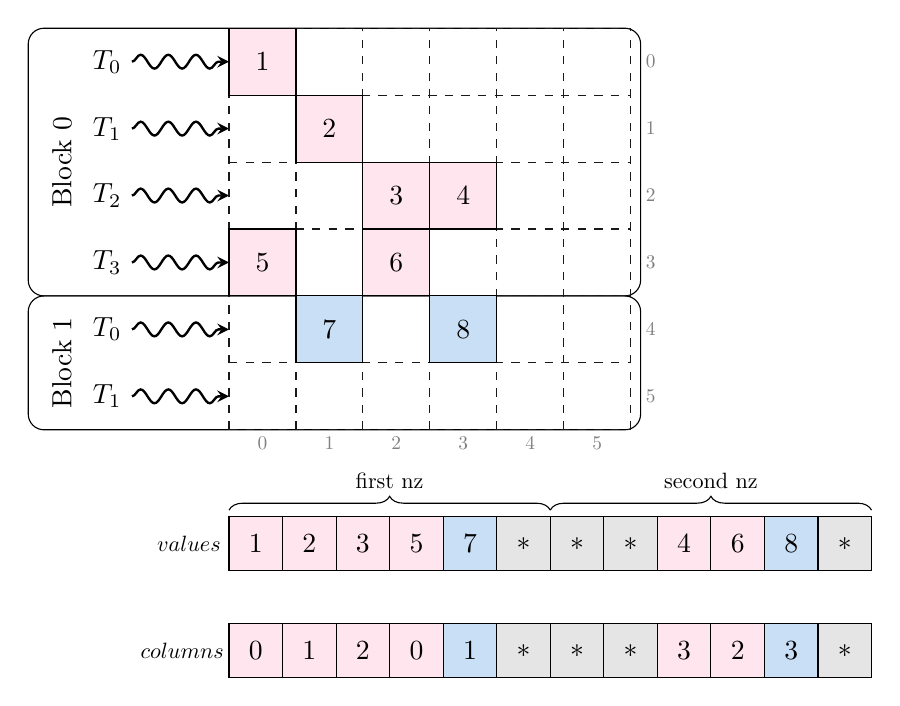
\begin{tikzpicture}[circ/.style = {circle, draw, inner sep=0pt, minimum size=3pt, outer sep=0pt, minimum size=6mm}, scale=0.85]

  \draw[round] (-3.0,4.0) rectangle (6.15,6.0);
  \draw[round] (-3.0,6.0) rectangle (6.15,10);

	\draw[draw=black,snake it,line width=0.30mm,>=stealth,->]   (-1.45,9.5) node [anchor=east] {$T_0$} -- (0,9.5);
	\draw[draw=black,snake it,line width=0.30mm,>=stealth,->]   (-1.45,8.5) node [anchor=east] {$T_1$} -- (0,8.5);
	\draw[draw=black,snake it,line width=0.30mm,>=stealth,->] (-1.45,7.5) node [anchor=east] {$T_2$} -- (0,7.5);
	\draw[draw=black,snake it,line width=0.30mm,>=stealth,->] (-1.45,6.5) node [anchor=east] {$T_3$} -- (0,6.5);

	\draw[draw=black,snake it,line width=0.30mm,>=stealth,->]   (-1.45,5.5) node [anchor=east] {$T_0$} -- (0,5.5);
	\draw[draw=black,snake it,line width=0.30mm,>=stealth,->]   (-1.45,4.5) node [anchor=east] {$T_1$} -- (0,4.5);
	
  \node[rotate=90] at (-2.5,8)   {Block 0};
  \node[rotate=90] at (-2.5,5.0) {Block 1};

  \foreach \y in {0,...,5} {
    \node[scale=0.7,text=gray] at (6.3,10.0 - 1.0*\y - 0.5) {\y};
  }

  \foreach \x in {0,...,5} {
    \node[scale=0.7,text=gray] at (1.0*\x + 0.5,3.8) {\x};
  }

  % Elements mesh
  \draw[step=1.0,black!90!white,thin,dashed,line width=0.4] (0.0,4.0) grid (6.0,10.0);

  \edef\esize{1.0}

  % ROW 0
  \edef\elementnum{1}
  \foreach \col in {0} {
    \draw[fill=r0d!60] (\col*\esize,9.0) rectangle (\col*\esize+\esize,10) node[pos=.5] {\elementnum};
    \pgfmathparse{int(\elementnum+1)}
    \xdef\elementnum{\pgfmathresult}
  }
  \foreach \col in {1} {
    \draw[fill=r0d!60] (\col*\esize,8.0) rectangle (\col*\esize+\esize,9) node[pos=.5] {\elementnum};
    \pgfmathparse{int(\elementnum+1)}
    \xdef\elementnum{\pgfmathresult}
  }
  \foreach \col in {2,3} {
    \draw[fill=r0d!60] (\col*\esize,7.0) rectangle (\col*\esize+\esize,8) node[pos=.5] {\elementnum};
    \pgfmathparse{int(\elementnum+1)}
    \xdef\elementnum{\pgfmathresult}
  }

  % ROW 4
  \foreach \col in {0,2} {
    \draw[fill=r0d!60] (\col*\esize,6.0) rectangle (\col*\esize+\esize,7) node[pos=.5] {\elementnum};
    \pgfmathparse{int(\elementnum+1)}
    \xdef\elementnum{\pgfmathresult}
  }

  % ROW 5
  \foreach \col in {1,3} {
    \draw[fill=r1d!60] (\col*\esize,5.0) rectangle (\col*\esize+\esize,6) node[pos=.5] {\elementnum};
    \pgfmathparse{int(\elementnum+1)}
    \xdef\elementnum{\pgfmathresult}
  }

  % RHS
  \edef\lasty{0}
  \edef\ynum{1}

  % =====================================================
  % ================== Data structures ================== 
  % =====================================================

  % RHS OFFSETS
  \edef\ybot{3.5}
  \edef\esize{0.8}

  \edef\xnum{0}
  \edef\lastblockoffset{0}
  \edef\lastyoffset{\ybot-\esize*0.8}

  % MATRIX DATA
  \pgfmathparse{\ybot-\esize*2}
  \xdef\ybot{\pgfmathresult}

  \node[scale=0.8] at (-0.6,\ybot+\esize/2) {$values$};

  % Col 0
  \edef\elementnum{0}
  \foreach \i in {1,2,3,5} {
    \draw[fill=r0d!60]  (\elementnum * \esize,\ybot) rectangle (\elementnum * \esize + \esize,\ybot+\esize) node[pos=0.5] {\i};
    \pgfmathparse{int(\elementnum+1)}
    \xdef\elementnum{\pgfmathresult}
  }
  \draw[fill=r1d!60]  (\elementnum * \esize,\ybot) rectangle (\elementnum * \esize + \esize,\ybot+\esize) node[pos=0.5] {7};
    \pgfmathparse{int(\elementnum+1)}
    \xdef\elementnum{\pgfmathresult}
  \draw[fill=gray!20] (\elementnum * \esize,\ybot) rectangle (\elementnum * \esize + \esize,\ybot+\esize) node[pos=0.5] {$*$};
    \pgfmathparse{int(\elementnum+1)}
    \xdef\elementnum{\pgfmathresult}
  \draw[fill=gray!20] (\elementnum * \esize,\ybot) rectangle (\elementnum * \esize + \esize,\ybot+\esize) node[pos=0.5] {$*$};
    \pgfmathparse{int(\elementnum+1)}
    \xdef\elementnum{\pgfmathresult}
  \draw[fill=gray!20] (\elementnum * \esize,\ybot) rectangle (\elementnum * \esize + \esize,\ybot+\esize) node[pos=0.5] {$*$};
    \pgfmathparse{int(\elementnum+1)}
    \xdef\elementnum{\pgfmathresult}
  \foreach \i in {4,6} {
    \draw[fill=r0d!60]  (\elementnum * \esize,\ybot) rectangle (\elementnum * \esize + \esize,\ybot+\esize) node[pos=0.5] {\i};
    \pgfmathparse{int(\elementnum+1)}
    \xdef\elementnum{\pgfmathresult}
  }
  \draw[fill=r1d!60]  (\elementnum * \esize,\ybot) rectangle (\elementnum * \esize + \esize,\ybot+\esize) node[pos=0.5] {8};
    \pgfmathparse{int(\elementnum+1)}
    \xdef\elementnum{\pgfmathresult}
  \draw[fill=gray!20] (\elementnum * \esize,\ybot) rectangle (\elementnum * \esize + \esize,\ybot+\esize) node[pos=0.5] {$*$};
    \pgfmathparse{int(\elementnum+1)}
    \xdef\elementnum{\pgfmathresult}
  % \foreach \i in {8,...,9} {
  %   \draw[fill=gray!20]  (\i * \esize,\ybot) rectangle (\i * \esize + \esize,\ybot+\esize) node[pos=0.5] {$*$};
  % }

  \pgfmathparse{\ybot-\esize*2}
  \xdef\ybot{\pgfmathresult}
  \node[scale=0.8] at (-0.7,\ybot+\esize/2) {$columns$};

  \edef\elementnum{0}
  \foreach \i in {0,1,2,0} {
    \draw[fill=r0d!60] (\elementnum * \esize,\ybot) rectangle (\elementnum * \esize + \esize,\ybot+\esize) node[pos=0.5] {\i};
    \pgfmathparse{int(\elementnum+1)}
    \xdef\elementnum{\pgfmathresult}
  }
  \foreach \i in {1} {
    \draw[fill=r1d!60] (\elementnum * \esize,\ybot) rectangle (\elementnum * \esize + \esize,\ybot+\esize) node[pos=0.5] {\i};
    \pgfmathparse{int(\elementnum+1)}
    \xdef\elementnum{\pgfmathresult}
  }
  \foreach \i in {1,...,3} {
    \draw[fill=gray!20] (\elementnum * \esize,\ybot) rectangle (\elementnum * \esize + \esize,\ybot+\esize) node[pos=0.5] {$*$};
    \pgfmathparse{int(\elementnum+1)}
    \xdef\elementnum{\pgfmathresult}
  }
  \foreach \i in {3,2} {
    \draw[fill=r0d!60] (\elementnum * \esize,\ybot) rectangle (\elementnum * \esize + \esize,\ybot+\esize) node[pos=0.5] {\i};
    \pgfmathparse{int(\elementnum+1)}
    \xdef\elementnum{\pgfmathresult}
  }
  \foreach \i in {3} {
    \draw[fill=r1d!60] (\elementnum * \esize,\ybot) rectangle (\elementnum * \esize + \esize,\ybot+\esize) node[pos=0.5] {\i};
    \pgfmathparse{int(\elementnum+1)}
    \xdef\elementnum{\pgfmathresult}
  }
  \foreach \i in {1} {
    \draw[fill=gray!20] (\elementnum * \esize,\ybot) rectangle (\elementnum * \esize + \esize,\ybot+\esize) node[pos=0.5] {$*$};
    \pgfmathparse{int(\elementnum+1)}
    \xdef\elementnum{\pgfmathresult}
  }

  \draw [brace] (0.0,2.8)  -- (6.0*\esize,2.8) node[toplabel] {first nz};
  \draw [brace] (6.0*\esize,2.8) -- (12.0*\esize,2.8) node[toplabel] {second nz};

  \end{tikzpicture}
  \caption{Example of ELL matrix format}
  \label{ell_format}
\end{figure}

Kernel for ELL matrix format is presented in the listing \ref{ell_implementation}. With element padding of the ELL format 
it's easy to get next row's element position by simply adding the number of rows in the matrix. The padding also fixes the
number of iteration for each thread, so there is no control flow divergence in warps. Elimination of control flow
divergence and enabling of memory coalescing allow ELL SpMV kernel to outperform CSR-Scalar implementation on many
matrices (tab. \ref{csr_ell_speedup_table}, fig. \ref{csr_ell_speedup_float} and \ref{csr_ell_speedup_double}). 

\begin{listing}[H]
\begin{minted}[linenos,tabsize=2]{cuda}
template <typename data_type>
__global__ void ell_spmv_kernel (
    unsigned int n_rows,
    unsigned int elements_in_rows,
    const unsigned int *col_ids,
    const data_type*data,
    const data_type*x,
    data_type*y)
{
  unsigned int row = blockIdx.x * blockDim.x + threadIdx.x;

  if (row < n_rows)
  {
    data_type sum = 0;
    for (unsigned int element = 0; element < elements_in_rows; element++)
    {
      const unsigned int element_offset = row + element * n_rows;
      sum += data[element_offset] * x[col_ids[element_offset]];
    }
    y[row] = sum;
  }
}
\end{minted}
\caption{ELL implementation}
\label{ell_implementation}
\end{listing}

\begin{table}[H]
	\centering
	\begin{tabular}{ |p{2.6cm}||p{1cm}|p{1cm}|p{1cm}|p{1cm}|  }
	 \hline
		& \multicolumn{2}{|c|}{float} & \multicolumn{2}{|c|}{double}\\
	 \hline
	 NNZ lower limit & avg & max & avg & max  \\
	 \hline
	 10000  & 6.73  & 35.47 & 5.57 & 27.92 \\
	 100000 & 11.16 & 35.47 & 8.44 & 27.92 \\
	 \hline
	\end{tabular}
	\caption{ELL speedup}
  \label{csr_ell_speedup_table}
\end{table}

\begin{figure}[H]
\centering
\subfloat[ELL speedup (float) \label{csr_ell_speedup_float}]  {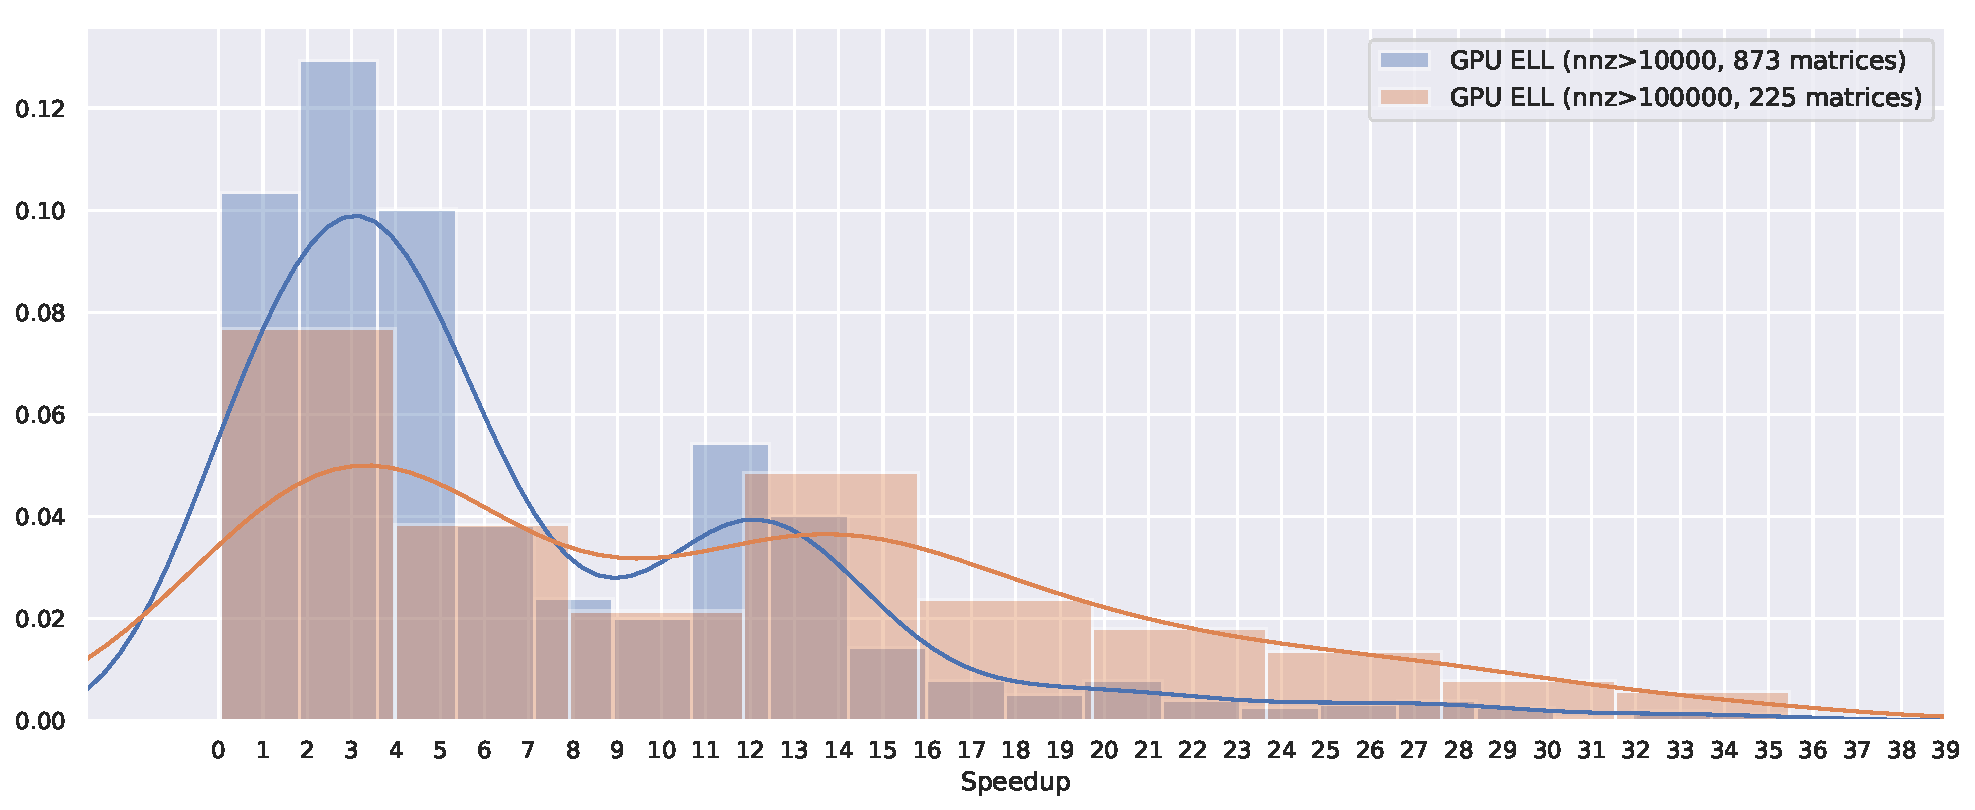
\includegraphics[width=1.0\textwidth]{img/csr_ell_float_dist.pdf}}
\qquad %
\subfloat[ELL speedup (double) \label{csr_ell_speedup_double}] {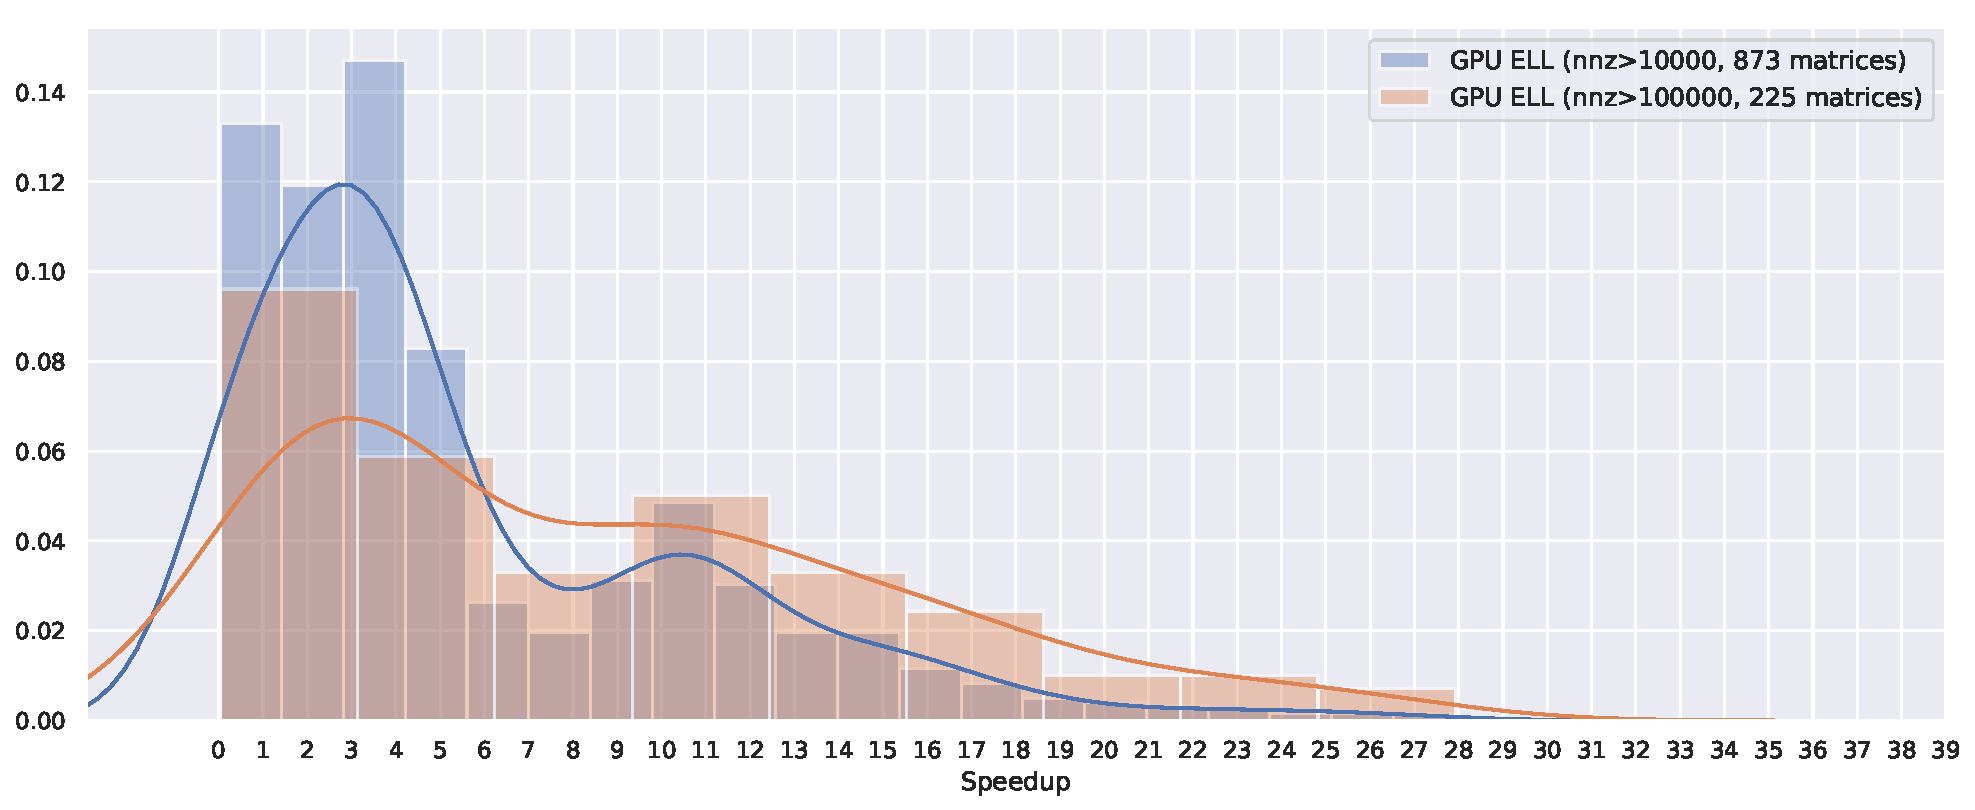
\includegraphics[width=1.0\textwidth]{img/csr_ell_double_dist.pdf}}
\end{figure}

The obvious disadvantage of ELL format consist in padding itself. In case of matrix with a few long rows, ELL format will result in 
excessive number of padded elements. There are a lot of matrices in Florida Collection, that coudn't fit into 8GB of my GPU because
of ELL's padding. In some cases it leads to the situation, where CSR-Scalar outperform ELL implementation. To eliminate this
issue, it's possible to remove long rows' extra nnz from ELL matrix into different matrix. It's important to note that
extracted matrix would have unordered scheme. Many rows will likely be missing from that scheme, so CSR using would be inefficient. 
One of the formats that could handle that case is COO.

\subsection{COO}

The coordinate (COO) matrix format is a the simpliest one. For each NZ it stores it's column and row indicies. Therefore, COO doesn't 
map elements in rows. That leads us to the necessity of atomic operations in COO kernel (list \ref{coo_implementation}).

\begin{listing}[H]
\begin{minted}[linenos,tabsize=2]{cuda}
template <typename data_type>
__global__ void coo_spmv_kernel (
    unsigned int n_elements,
    const unsigned int *col_ids,
    const unsigned int *row_ids,
    const data_type *data,
    const data_type *x,
    data_type *y)
{
  unsigned int element = blockIdx.x * blockDim.x + threadIdx.x;

  if (element < n_elements)
    atomicAdd (y + row_ids[element], data[element] * x[col_ids[element]]);
}
\end{minted}
\caption{COO implementation}
\label{coo_implementation}
\end{listing}

\begin{table}[H]
	\centering
	\begin{tabular}{ |p{2.6cm}||p{1cm}|p{1cm}|p{1cm}|p{1cm}|  }
	 \hline
		& \multicolumn{2}{|c|}{float} & \multicolumn{2}{|c|}{double}\\
	 \hline
	 NNZ lower limit & avg & max & avg & max  \\
	 \hline
	 10000  & 6.96  & 54.15 & 7.37  & 37.83 \\
	 100000 & 10.55 & 54.15 & 11.69 & 37.83 \\
	 \hline
	\end{tabular}
	\caption{COO speedup}
  \label{csr_coo_speedup_table}
\end{table}

\begin{figure}[H]
\centering
\subfloat[COO speedup (float) \label{csr_coo_speedup_float}]  {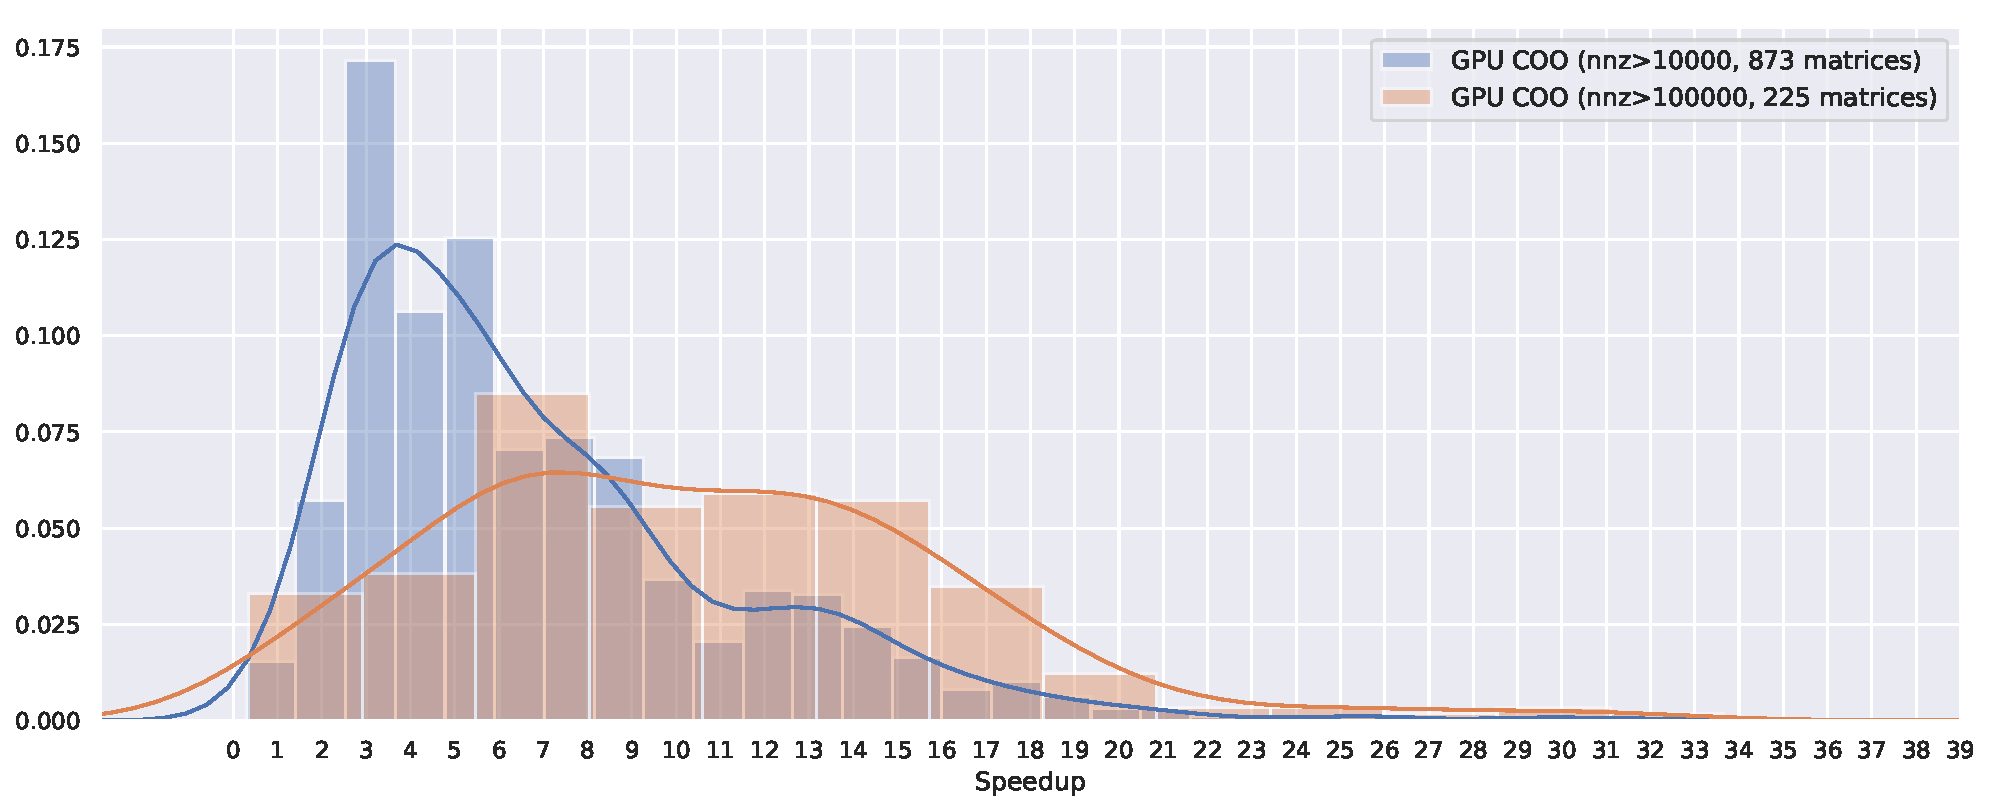
\includegraphics[width=1.0\textwidth]{img/coo_float_dist.pdf}}
\qquad %
\subfloat[COO speedup (double) \label{csr_coo_speedup_double}] {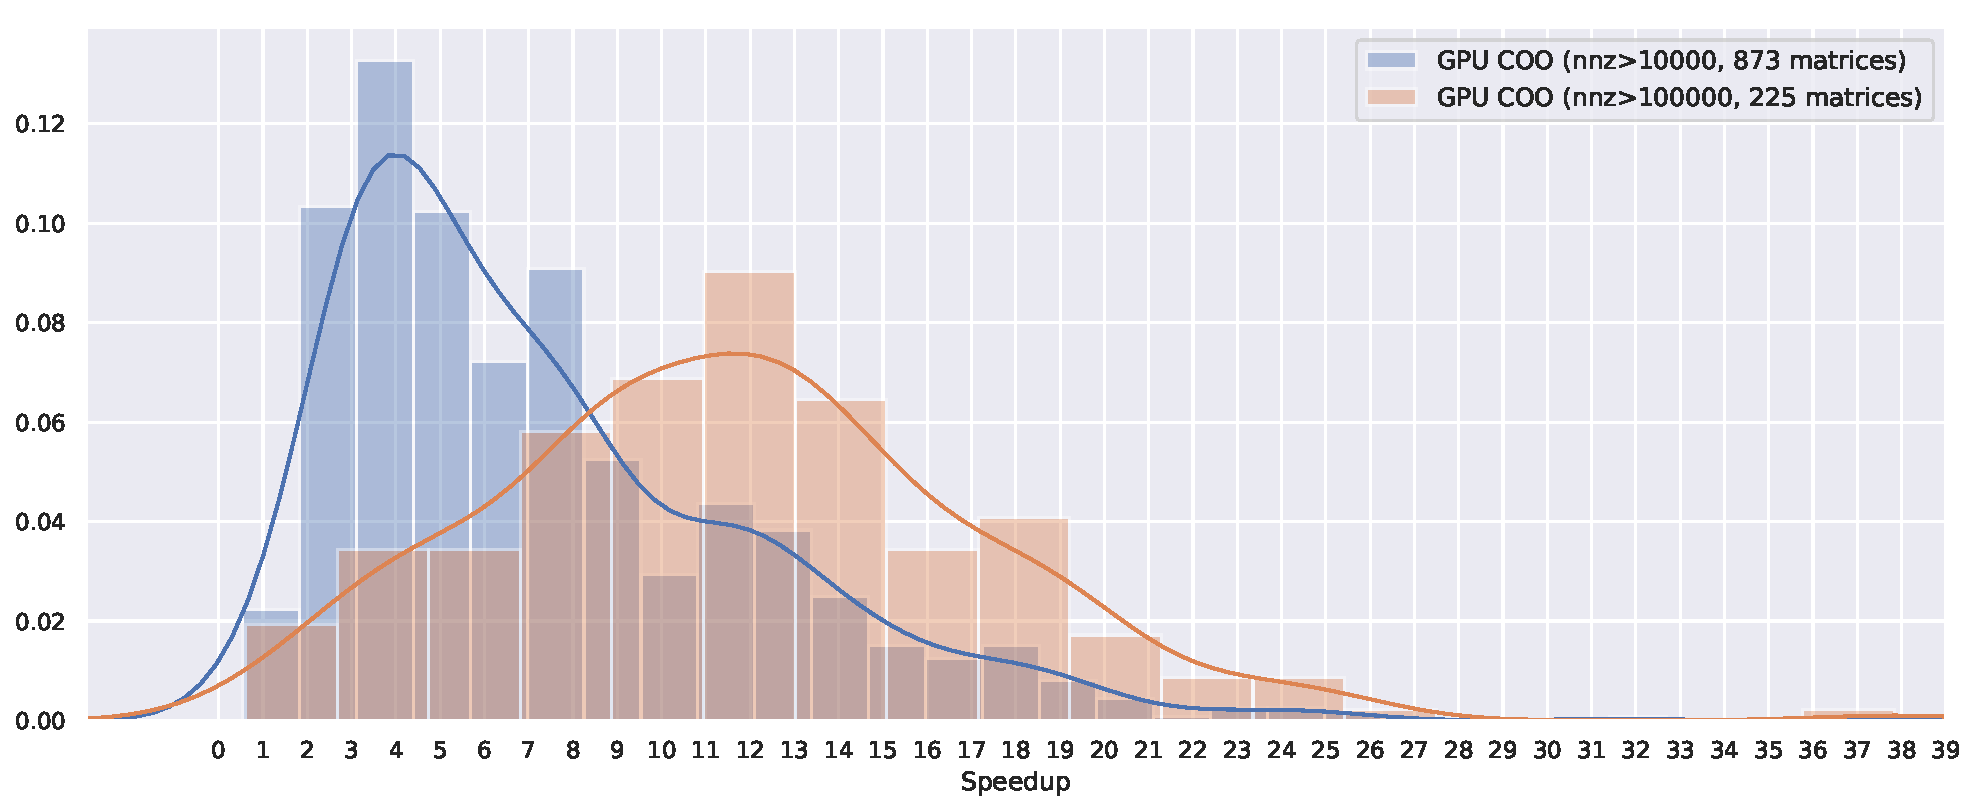
\includegraphics[width=1.0\textwidth]{img/coo_double_dist.pdf}}
\end{figure}

COO SpMV implementation works at the granularity of threads per element (\ref{coo_implementation}). Atomic updates to the result vector 
reduce performance. The wider rows in COO format, the more serialized SpMV is. This fact can be noticed from figure \ref{coo_nnzpr}. To improve
performance of this format it's possible to slice the matrix info chunks with the rows count that fits into shared memory.

\begin{figure}[H]
\centering
  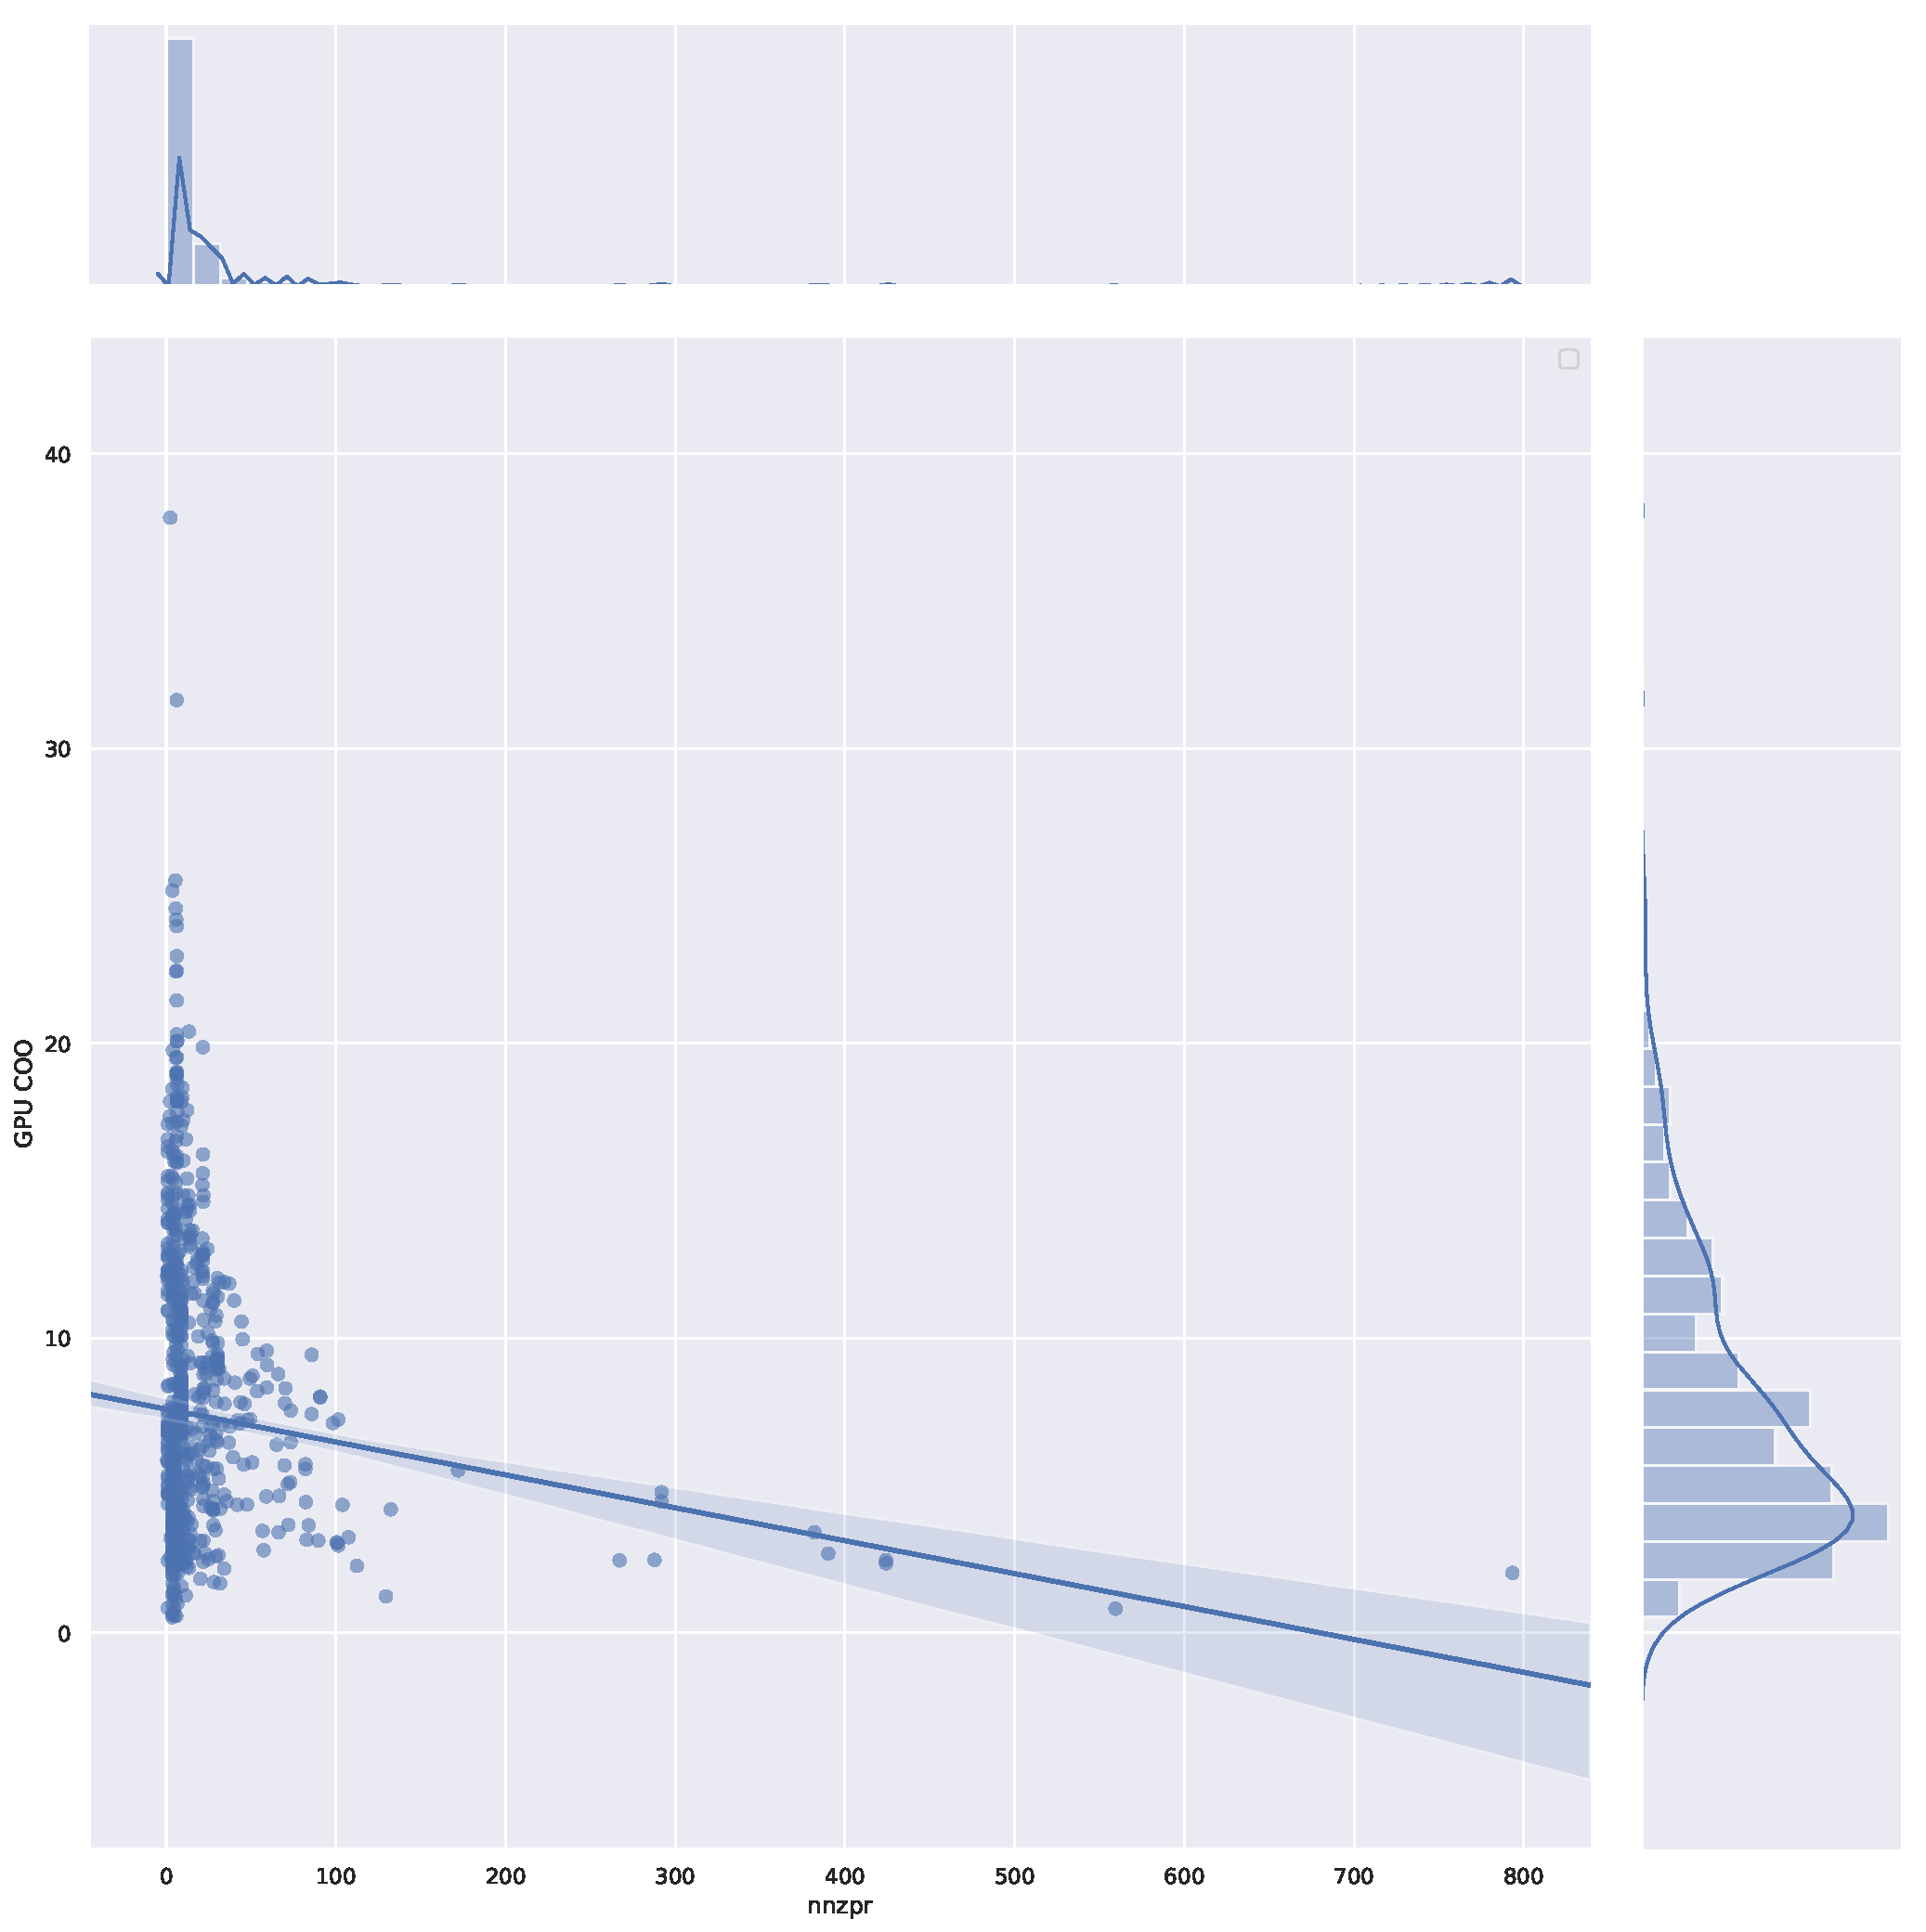
\includegraphics[width=1.0\textwidth]{img/coo_nnzpr.pdf}
  \caption{The dependence of the COO parameter on the average NNZ}
  \label{coo_nnzpr}
\end{figure}

Matrix format that uses shared memory to improve atomic operations performance in COO SpMV is called Sliced COO (SCOO).
To reduce shared memory bank conflicts, SCOO allows multiple lanes in the shared memory for updating the intermediate results of a
single row. Reducing slice size increases lanes size and thus more shared memory lanes are available.

\begin{table}[H]
	\centering
	\begin{tabular}{ |p{2.6cm}||p{1cm}|p{1cm}|p{1cm}|p{1cm}|  }
	 \hline
		& \multicolumn{2}{|c|}{float} & \multicolumn{2}{|c|}{double}\\
	 \hline
	 NNZ lower limit & avg & max & avg & max  \\
	 \hline
	 10000  & 6.82  & 38.63 & 4.60 & 26.78 \\
	 100000 & 12.46 & 38.63 & 7.43 & 26.78 \\
	 \hline
	\end{tabular}
	\caption{SCOO speedup}
  \label{scoo_speedup_table}
\end{table}




\subsection{Hybrid}
It's possible to use ELL matrix format on regular part of the matrix and COO on the elements removed from extra-long rows. This scheme
significantly reduces the number of padded elements in ELL format. This approach is often called as hybrid. There is different options
for combining results of ELL and COO SpMV. In this post I use atomic case (list. \ref{hybrid_implementation}).

\begin{listing}[H]
\begin{minted}[linenos,tabsize=2]{cuda}
template <typename data_type>
__global__ void hybrid_spmv_kernel (
    unsigned int n_rows,
    unsigned int n_elements,
    unsigned int elements_in_rows,
    const unsigned int *ell_col_ids,
    const unsigned int *col_ids,
    const unsigned int *row_ids,
    const data_type *ell_data,
    const data_type *coo_data,
    const data_type *x,
    data_type *y)
{
  const unsigned int idx = blockIdx.x * blockDim.x + threadIdx.x;

  if (idx < n_rows)
  {
    const unsigned int row = idx;

    data_type sum = 0;
    for (unsigned int element = 0; element < elements_in_rows; element++)
    {
      const unsigned int element_offset = row + element * n_rows;
      sum += ell_data[element_offset] * x[ell_col_ids[element_offset]];
    }
    atomicAdd (y + row, sum);
  }

  for (unsigned int element = idx; element < n_elements; element += blockDim.x * gridDim.x)
  {
    const data_type sum = coo_data[element] * x[col_ids[element]];
    atomicAdd (y + row_ids[element], sum);
  }
}
\end{minted}
\caption{Hybrid implementation}
\label{hybrid_implementation}
\end{listing}

Althought, the average performance results (tab. \ref{hyb_speedup_table}, fig. \ref{hyb_scoo_speedup_float} and \ref{hyb_scoo_speedup_double}) are
quite close to CSR-Adaptive SpMV, Hybrid format requires extra actions of splitting matrix, which might require rewriting of matrix calculation code base.

\begin{table}[H]
	\centering
	\begin{tabular}{ |p{2.6cm}||p{1cm}|p{1cm}|p{1cm}|p{1cm}|  }
	 \hline
		& \multicolumn{2}{|c|}{float} & \multicolumn{2}{|c|}{double}\\
	 \hline
	 NNZ lower limit & avg & max & avg & max  \\
	 \hline
	 10000  & 7.73  & 38.62 & 6.51  & 25.96 \\
	 100000 & 14.92 & 38.62 & 11.59 & 25.96 \\
	 \hline
	\end{tabular}
	\caption{HYB speedup}
  \label{hyb_speedup_table}
\end{table}

\begin{figure}[H]
\centering
\subfloat[HYB speedup (float) \label{hyb_scoo_speedup_float}]  {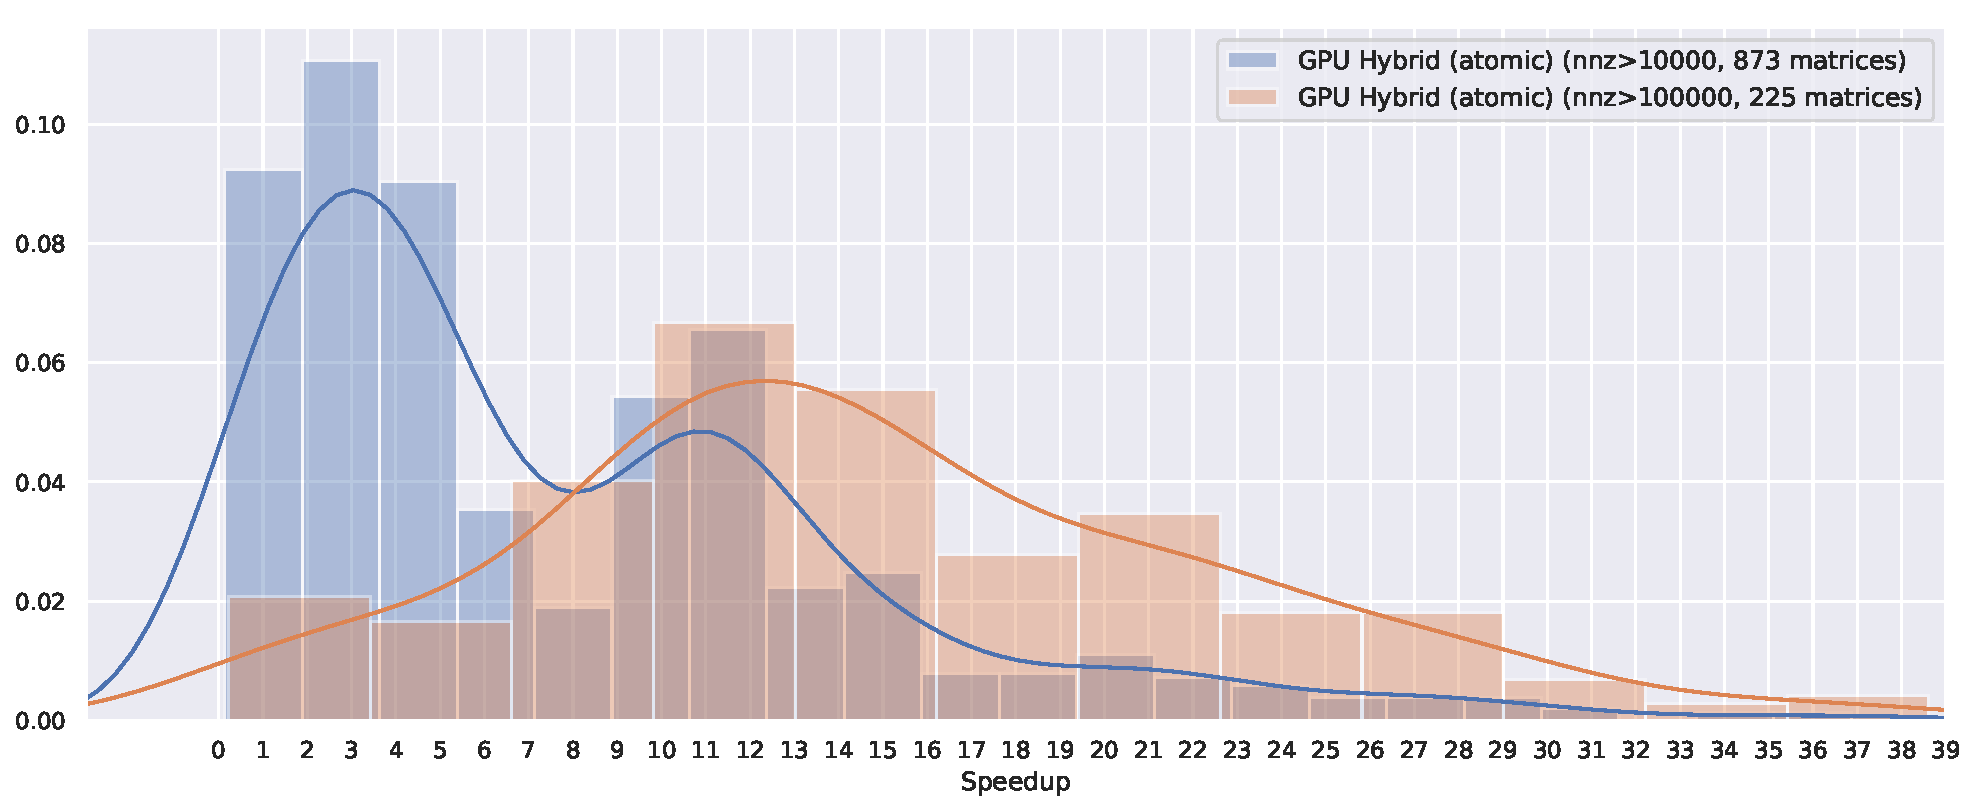
\includegraphics[width=1.0\textwidth]{img/hybrid_float_dist.pdf}}
\qquad %
\subfloat[HYB speedup (double) \label{hyb_scoo_speedup_double}] {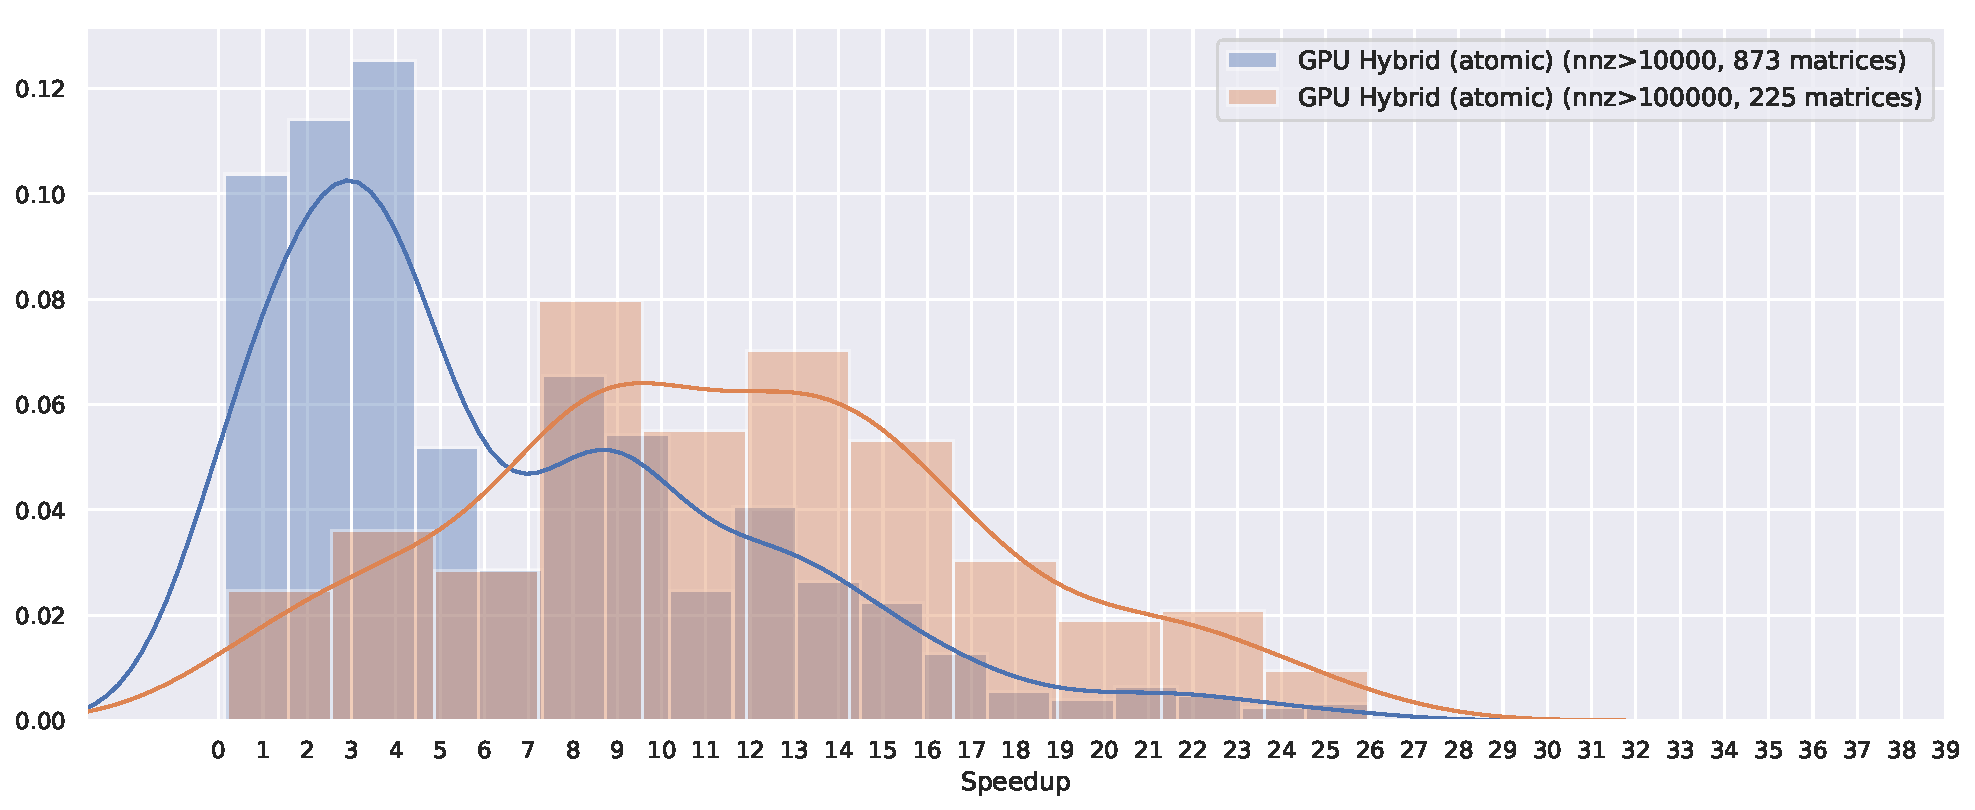
\includegraphics[width=1.0\textwidth]{img/hybrid_double_dist.pdf}}
\end{figure}




\section{Conclusion}
Write your conclusion here.

\begin{table}[H]
\centering
\begin{tabular}{ c c c c }
  airfoil\_2d & cavity21 & coater2 & lhr07 \\
  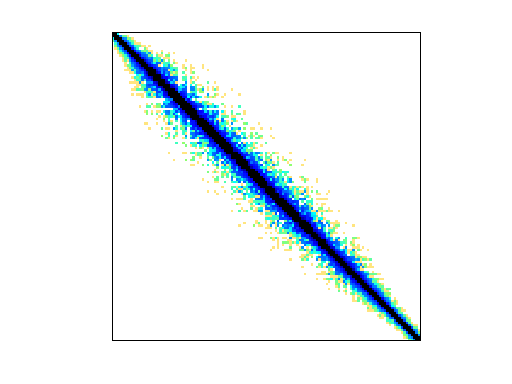
\includegraphics[width=0.2\textwidth]{img/matrices/airfoil_2d.png} & 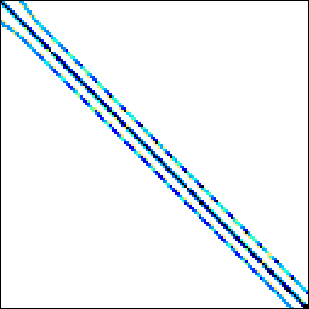
\includegraphics[width=0.2\textwidth]{img/matrices/cavity21.png} & 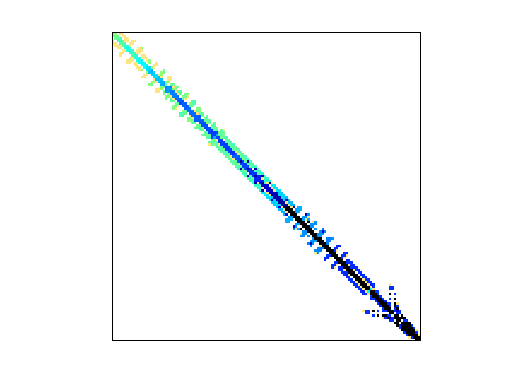
\includegraphics[width=0.2\textwidth]{img/matrices/coater2.png} & 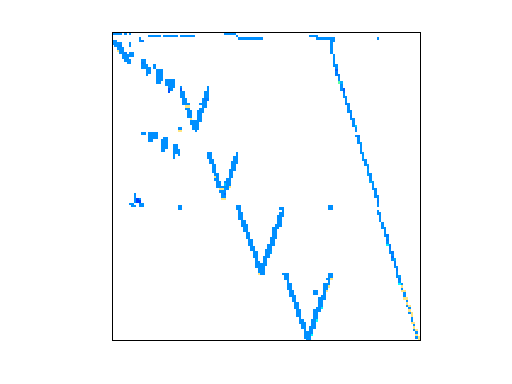
\includegraphics[width=0.2\textwidth]{img/matrices/lhr07.png} \\
  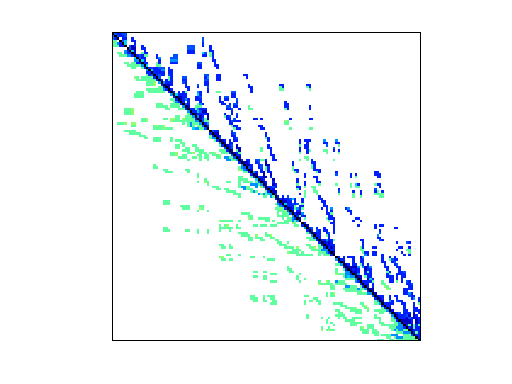
\includegraphics[width=0.2\textwidth]{img/matrices/cage10.png} & 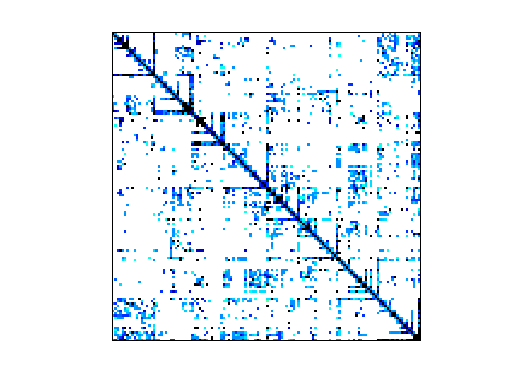
\includegraphics[width=0.2\textwidth]{img/matrices/ASIC_100ks.png} & 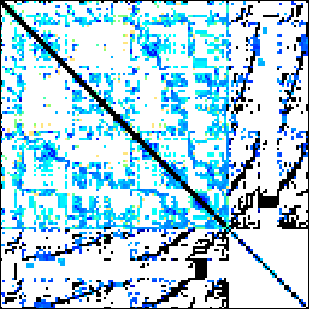
\includegraphics[width=0.2\textwidth]{img/matrices/scircuit.png} & 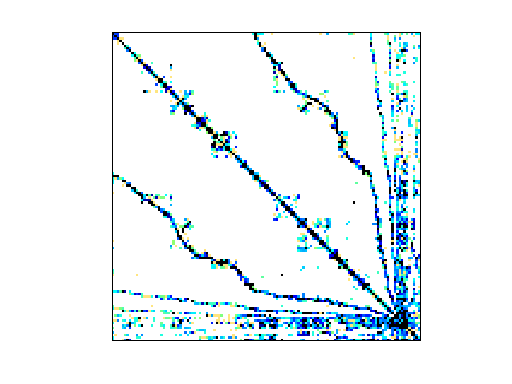
\includegraphics[width=0.2\textwidth]{img/matrices/hvdc1.png} \\
  cage10 & ASIC\_100ks & scircuit & hvdc1 \\
\end{tabular}
\end{table}

\end{document}
